\documentclass[10pt,aps,onecolumn,superscriptaddress]{revtex4-2}

\usepackage[T1]{fontenc}
\usepackage[utf8]{inputenc}
\usepackage[english]{babel}

\usepackage{amsfonts,amsbsy,amssymb,amsmath}
\usepackage{graphicx,float}
\usepackage{hyperref}
\hypersetup{
    colorlinks=true,
    linkcolor=blue,
    filecolor=magenta,      
    urlcolor=cyan,
}

\graphicspath{{notebooks/figures/}}

\bibliographystyle{apsrev4-2}

\begin{document}

\title{Chemical Reaction Dynamics \\ on the Cirque Potential Energy Surface}

%\author{Broncio Aguilar Sanjuan}
%\email{broncio.aguilarsanjuan@bristol.ac.uk}
%\affiliation{School of Mathematics, University of Bristol, \\ Fry Building, Woodland Road, Bristol, BS8 1UG, United Kingdom.}
%
%\author{Francisco Gonz\'alez Montoya}
%\email{fg16704@bristol.ac.uk}
%\affiliation{School of Mathematics, University of Bristol, \\ Fry Building, Woodland Road, Bristol, BS8 1UG, United Kingdom.}
%
%\author{V\'ictor J. Garc\'ia-Garrido}
%\email{vjose.garcia@uah.es}
%\affiliation{Departamento de F\'isica y Matem\'aticas, Universidad de Alcal\'a, \\ Alcal\'a de Henares, 28871, Spain.}
%
%\author{Stephen Wiggins}
%\email{s.wiggins@bristol.ac.uk}
%\affiliation{School of Mathematics, University of Bristol, \\ Fry Building, Woodland Road, Bristol, BS8 1UG, United Kingdom.}


\begin{abstract}

In this paper we explore the bifurcation scenario when the energy is increased.

% Energy before the threshold E < 0,  Closed system
% Energies corresponding to the bifurcation of the periodic orbits type I , II , III, Open system
%% Conjecture E_I > E_II > E_III

\end{abstract}

\maketitle

\noindent\textbf{Keywords:} Phase space structure, Chemical reaction dynamics, Roaming, Lagrangian descriptors, 

\section{Introduction}

\section{The Cirque Potential Energy Surface Model}

In this section we introduce the Cirque potential energy surface (PES) that we will analyze in this work. This model is constructed from the superposition of two van der Waals potentials that are centered at symmetrically located points with respect to the origin. This approach is similar to that followed in \cite{GonzalezMontoya2020} to generate a double-Morse potential. For the single van der Waals potential energy we use the expression introduced in \cite{Soley2018} which models the long-range interaction describing dipole-dipole attraction between neutral molecules/atoms. This potential has the structure: 
\begin{equation}
W(r) = -\dfrac{C}{(\beta r^2 + \alpha)^3}
\label{eq:vdw-single}
\end{equation}
where $r$ is the radial coordinate in the plane, $C$ is the van der Waals dispersion coefficient, $\alpha$ is a parameter that removes the singularity from the origin, $r = 0$, and $\beta$ is the characteristic length parameter. They are all positive constants. The potential's minimum is located at the origin, i.e. $r = r_e = 0$, with energy: 
\begin{equation}
W\left(r_e\right) = - \dfrac{C}{\alpha^3}
\end{equation}
Note that the potential has axial-symmetry since it only depends on the radial distance. Moreover, when $r \rightarrow + \infty$ the leading order form of the potential is:
\begin{equation}
W(r) \sim - \frac{C}{\beta^3 r^6}
\end{equation}

In this work we have adopted the convention of writing this model potential in an alternative way so that its parameters have a geometrical interpretation regarding the shape of the potential energy function. Consider the function:
\begin{equation}
W(r) = - \dfrac{W_0 \, k^6}{\left(r^2 + k^2\right)^3}
\label{eq:heller_pes}
\end{equation}
It is straightforward to show that $W_0$ represents the depth of the potential well located at the origin with respect to the dissociation energy, which is given by:
\begin{equation}
W_{\infty} = \lim_{r \to \infty} W(r) = 0
\end{equation}
Moreover, the parameter $k$ determines the half-width of the well as measured at the energy level corresponding to one eighth the energy of the minimum at the bottom of the well. The effect of the parameters $k$ and $W_0$ on the geometry of the potential is represented in Fig. \ref{fig:heller_pes}. We can easily shift the PES in Eq. \eqref{eq:heller_pes} to any point $\mathbf{r}_0 = (x_0,y_0)$ in configuration space. To d so, consider the position vector $\mathbf{r} = (x,y)$ and define the function:
\begin{equation}
W_{\mathbf{r}_0}(\mathbf{r}) = W(\mathbf{r} - \mathbf{r}_0) = - \dfrac{W_0 \, k^6}{\left( |\mathbf{r} - \mathbf{r}_0|^2 + k^2\right)^3} = - \dfrac{W_0 \, k^6}{\left(\left(x-x_0\right)^2 + \left(y-y_0\right)^2 + k^2\right)^3}
\end{equation}
Therefore, the double van der Waals PES used to model the Cirque energy landscape can be  constructed by means of choosing two points on the $x$-axis separated the same distance $d$ from the origin, that is, $\mathbf{r}_{1,2} = (\pm d,0)$, and superposing their potentials so that:
\begin{equation}
V(\mathbf{r}) \equiv V(x,y) =  W_{\mathbf{r}_1}(\mathbf{r}) + W_{\mathbf{r}_2}(\mathbf{r})
= - W_0 \, k^6 \left[\dfrac{1}{\left(\left(x - d\right)^2 + y^2 + k^2\right)^3} + \dfrac{1}{\left(\left(x + d\right)^2 + y^2 + k^2\right)^3} \right]
\label{eq:double_vdw}
\end{equation}

\begin{figure}[htbp]
	\centering
	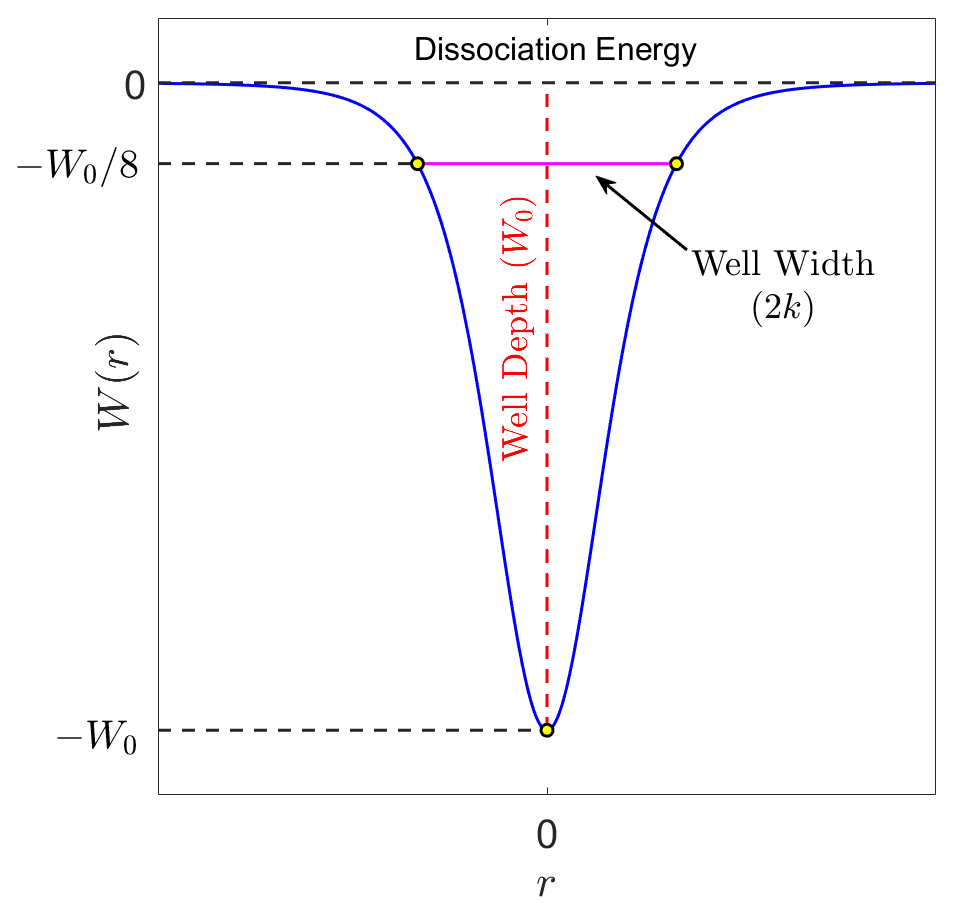
\includegraphics[scale=0.28]{heller_potFunc_new2.png}
	\caption{Geometrical interpretation of the parameters determining the shape of the PES in Eq. \eqref{eq:heller_pes}.}
	\label{fig:heller_pes}
\end{figure}


\begin{figure}[htbp]
	A)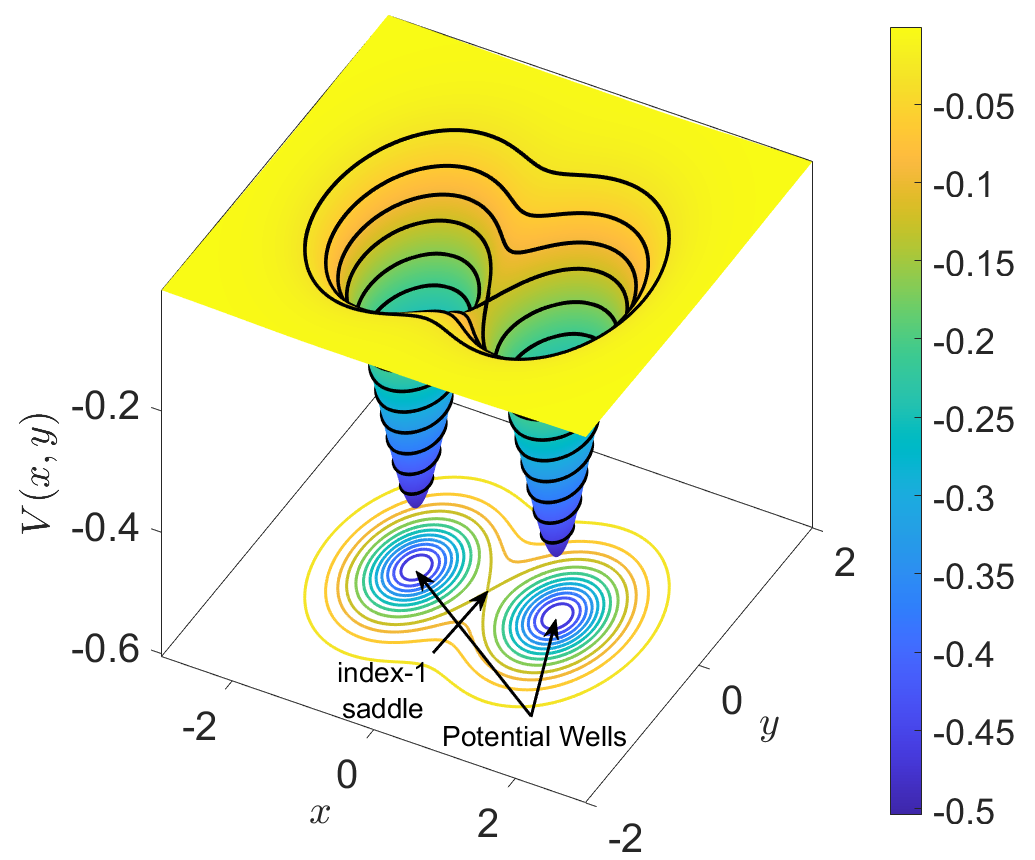
\includegraphics[scale=0.28]{PES_Cirque_w0_1div2_k_1_d_1.png}
	B)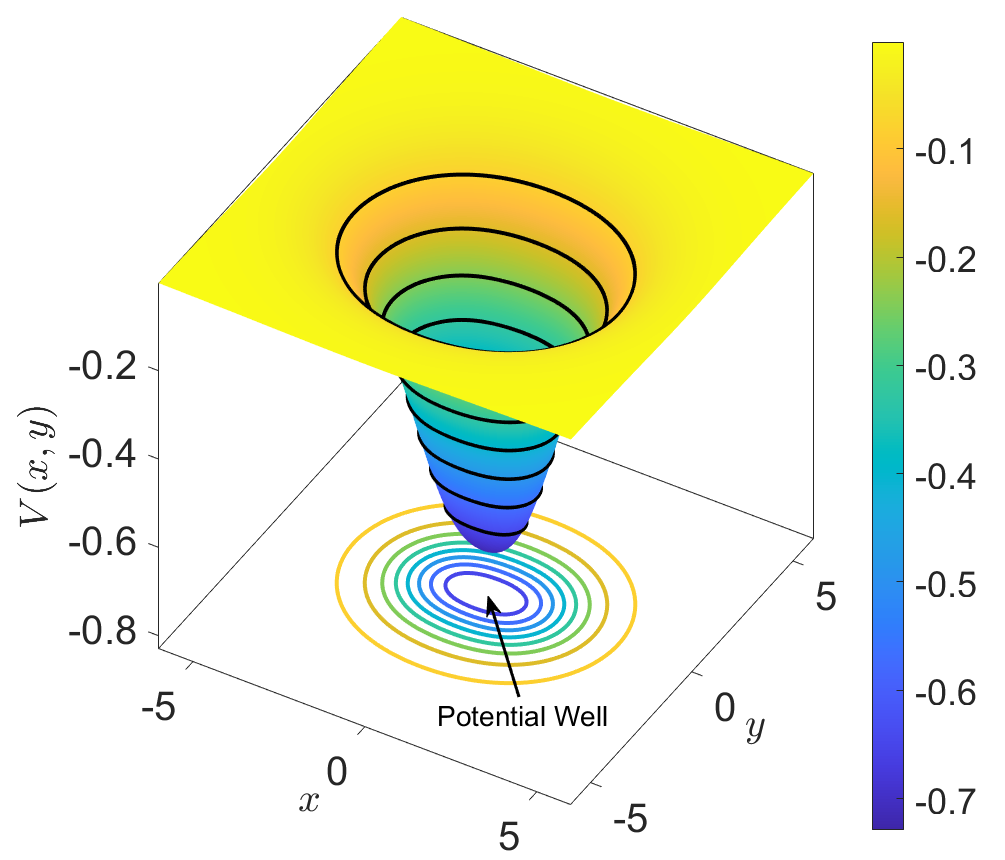
\includegraphics[scale=0.28]{PES_Cirque_w0_1div2_k_3_d_1.png}
	C)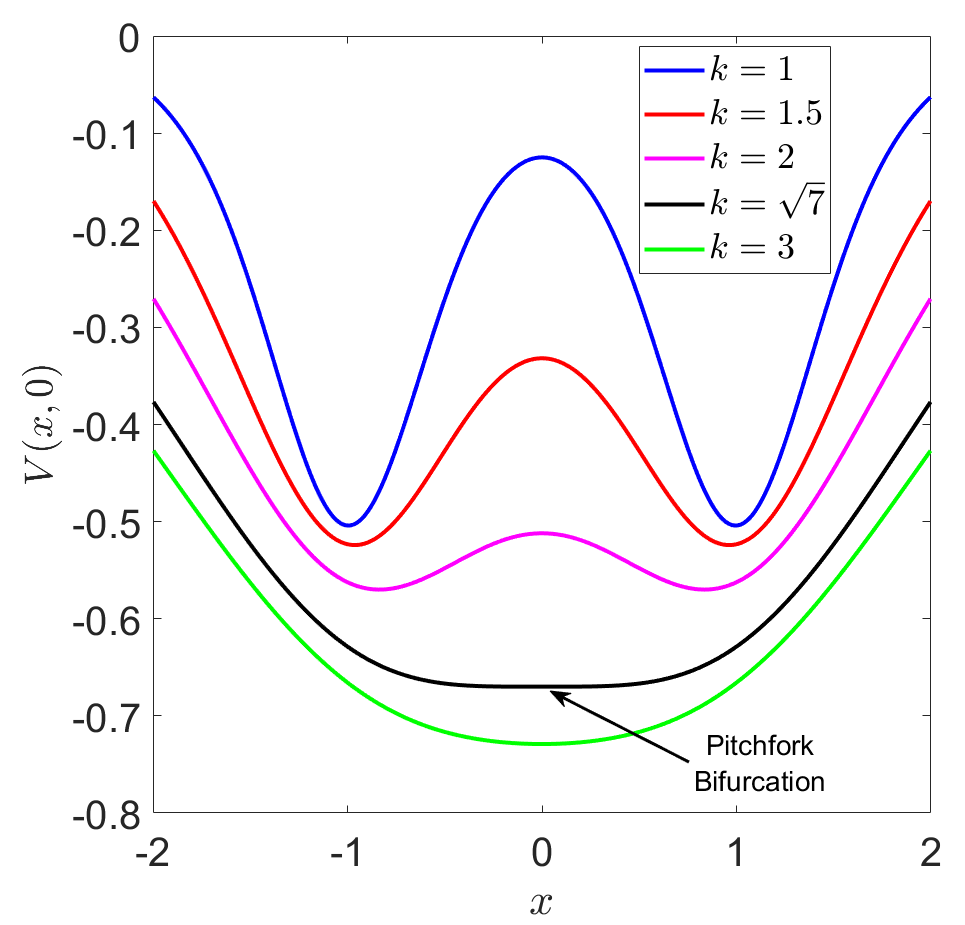
\includegraphics[scale=0.25]{pitcforkBif.png}
	\caption{Double van der Waals PES in Eq. \eqref{eq:double_vdw} for the model parameters: A) $W_0 = 1/2$, $k = 1$, $d = 1$; B) $W_0 = 1/2$, $k = 3$, $d = 1$; C) Pitchfork bifurcation of the PES along the $x$-axis for $W_0 = 1/2$ and $d = 1$, as the well width parameter $k$ is varied.}
	\label{fig:double_vdw_PES}
\end{figure}


%\begin{figure}[htbp]
%    A)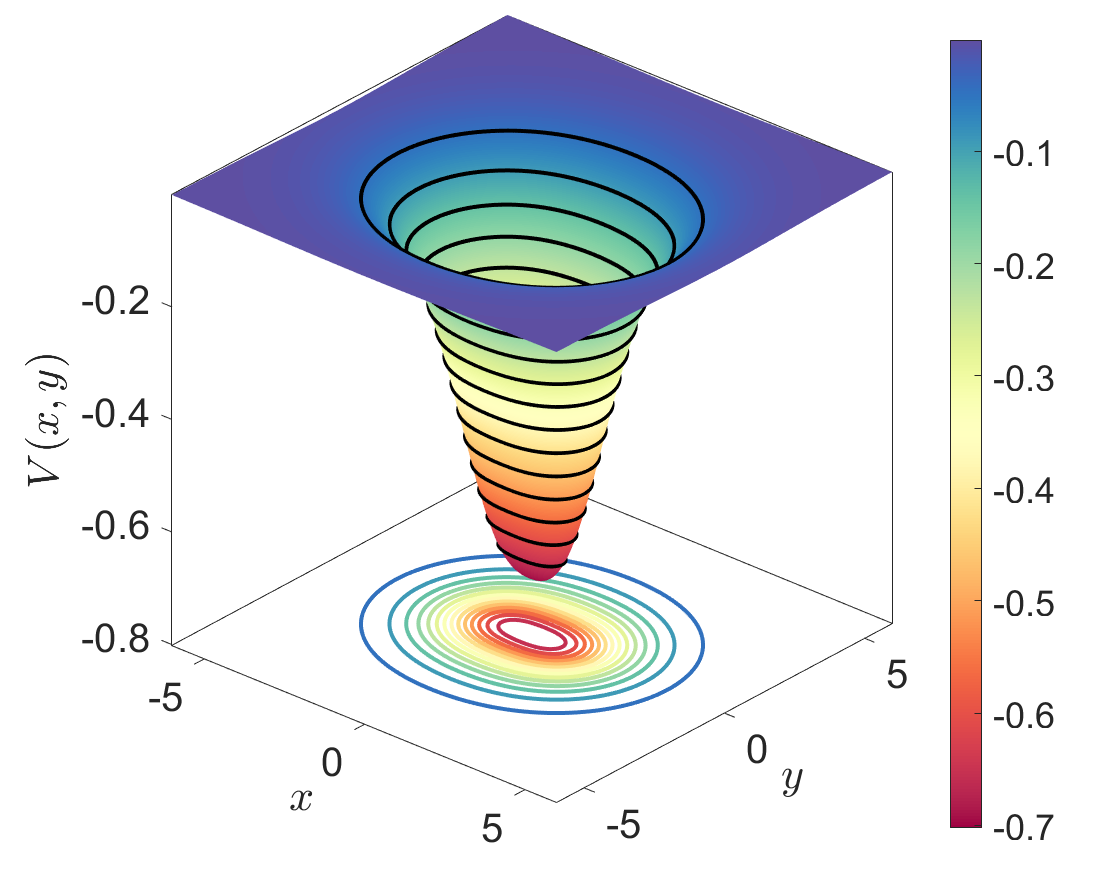
\includegraphics[scale=0.24]{CirquePES_c_1div2_a_1_b_1div8_d_1.png}
%    B)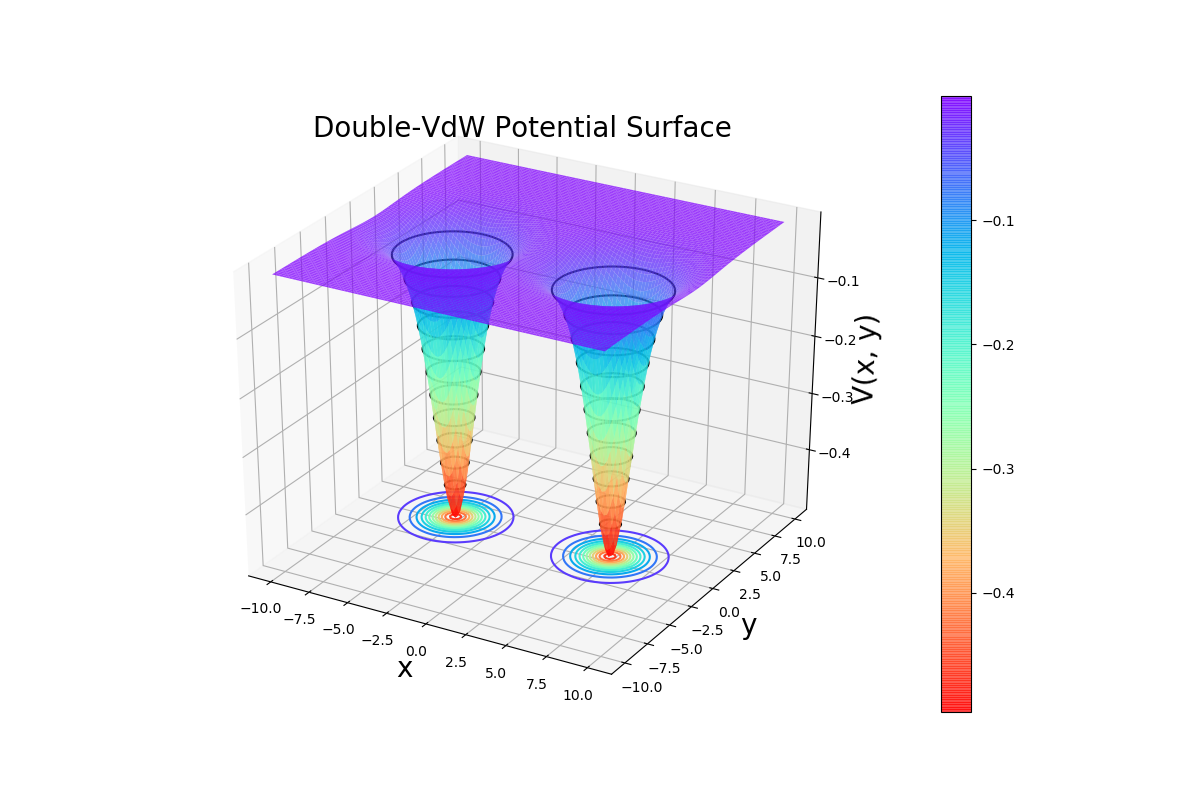
\includegraphics[scale=0.33]{double-vdw_surface.png}
%    \caption{Double van der Waals PES in Eq. \eqref{eq:vdw-single} for the model parameters: A) $C = 1/2$, $\alpha = 1$, $\beta = 1/8$ and $d = 1$; B) $C = 1/2$, $\alpha = 1$, $\beta = 1/8$, and $d = 5$.}
%    \label{fig:vdw-single_surface}
%\end{figure}

The two degrees-of-freedom (DoF) Hamiltonian for the Cirque potential energy surface is defined as the classical sum of kinetic plus potential energy:
\begin{equation}
H(x,y,p_x,p_y) = \dfrac{p_x^2}{2 m_1} + \dfrac{p_y^2}{2 m_2} + V(x,y)
\label{eq:hamil}
\end{equation}
where $m_1$ and $m_2$ are the masses in the $x$ and $y$ DoF respectively. Hamilton's equations that determine the systems dynamical evolution are given by:
\begin{equation}
\begin{cases}
\dot{x} = \dfrac{\partial H}{\partial p_x} = \dfrac{p_x}{m_1} \\[.5cm]
\dot{y} = \dfrac{\partial H}{\partial p_y} = \dfrac{p_y}{m_2} \\
\dot{p}_x = - \dfrac{\partial H}{\partial x} = - \dfrac{\partial V}{\partial x} = - 6 W_0 \, k^6 \left[\dfrac{x - d}{\left(\left(x - d\right)^2 + y^2 + k^2\right)^4} + \dfrac{x + d}{\left(\left(x + d\right)^2 + y^2 + k^2\right)^4}\right] \\[.8cm]
\dot{p}_y = - \dfrac{\partial H}{\partial y} = - \dfrac{\partial V}{\partial y} = - 6 W_0 \, k^6 y \left[\dfrac{1}{\left(\left(x - d\right)^2 + y^2 + k^2\right)^4} + \dfrac{1}{\left(\left(x + d\right)^2 + y^2 + k^2\right)^4}\right]
\end{cases}
\label{eq:ham_eq}
\end{equation}
In this work we will consider the situation where both DoF have unit mass, that is $m_1 = m_2 = 1$. The equilibrium points $\mathbf{x}_e = (x_e,y_e,p_{x,e},p_{y,e})$ of the dynamical system given above are contained in configuration space, since $p_{x,e} = p_{y,e} = 0$, and they are also critical points of the PES, that is $\nabla V (x_e,y_e) = \mathbf{0}$. It is straightforward to check that under these conditions, the points have to satisfy:
\begin{equation}
y_e = 0 \quad , \quad \left(x_e - d\right) \left[\left(x_e + d\right)^2 + k^2\right]^4 + \left(x_e + d\right) \left[\left(x_e - d\right)^2 + k^2\right]^4 = 0 
\label{eq:eq_pts}
\end{equation}
It is straightforward to show that $x_e = 0$ is always a solution to the equation above, and therefore the origin is always an equilibrium point of Hamilton's equations for this system. Moreover, there is also an equilibrium point located at infinity. Regarding the presence of other equilibria, this depends critically on the model parameters, and if they exist, their coordinates are of the form $\mathbf{x}_e = (x_e(k,d),0,0,0)$. 

The linear stability of these equilibrium points is determined by the eigenvalues of the Jacobian matrix given by the linearization of Eq. \eqref{eq:ham_eq} about each of the points. In order to construct the Jacobian, we need to compute the second order partial derivatives that characterize the Hessian matrix of the PES:
\begin{equation}
\begin{cases}
\dfrac{\partial^{\,	2} V}{\partial x^2} = 6 \, W_0 \, k^6 \left[\dfrac{-7\left(x - d\right)^2 + y^2 + k^2}{\left(\left(x - d\right)^2 + y^2 + k^2\right)^5} + \dfrac{-7\left(x + d\right)^2 + y^2 + k^2}{\left(\left(x + d\right)^2 + y^2 + k^2\right)^5} \right] \\[.8cm]

\dfrac{\partial^{\,	2} V}{\partial y^2} = 6 \, W_0 \, k^6 \left[\dfrac{\left(x - d\right)^2 - 7 y^2 + k^2}{\left(\left(x - d\right)^2 + y^2 + k^2\right)^5} + \dfrac{\left(x + d\right)^2 - 7y^2 + k^2}{\left(\left(x + d\right)^2 + y^2 + k^2\right)^5} \right] \\[.8cm]

\dfrac{\partial^{\,	2} V}{\partial x \partial y} = - 48 \, W_0 \, k^6 \, y \left[\dfrac{x - d}{\left(\left(x - d\right)^2 + y^2 + k^2\right)^5} + \dfrac{x + d}{\left(\left(x + d\right)^2 + y^2 + k^2\right)^5}\right]
\end{cases}
\label{eq:second_pder}
\end{equation}
We take a look now at the Hessian matrix of the PES evaluated at the origin:
\begin{equation}
\text{Hess}_{V}(0,0) = \begin{pmatrix}
\dfrac{\partial^{\,	2} V}{\partial x^2}(0,0) & \dfrac{\partial^{\,	2} V}{\partial x \partial y}(0,0) \\[.4cm]
\dfrac{\partial^{\,	2} V}{\partial y \partial x}(0,0) & \dfrac{\partial^{\, 2} V}{\partial y^2}(0,0)
\end{pmatrix} = \begin{pmatrix}
\dfrac{12 W_0 \, k^6 \left(k^2 - 7 d^2\right)}{\left(d^2 + k^2\right)^5} & 0 \\[.5cm]
0 & \dfrac{12 W_0 \, k^6}{\left(d^2 + k^2\right)^4}
\end{pmatrix}
\end{equation}
The linear stability of the origin is characterized by the nature of the eigenvalues of the Jacobian matrix:
\begin{equation}
J(0,0) = \begin{pmatrix}
\mathbb{O}_2 & \hspace{.2cm} \mathbb{I}_2 \hspace{.1cm} \\[.3cm]
-\text{Hess}_{V}(0,0) & \hspace{.2cm} \mathbb{O}_2 \hspace{.1cm}
\end{pmatrix} = \begin{pmatrix}
0 & 0 & \hspace{.5cm} 1 & \hspace{.5cm} 0 \hspace{.2cm} \\[.4cm]
0 & 0 & \hspace{.5cm} 0 & \hspace{.5cm} 1 \hspace{.2cm} \\[.4cm]
\dfrac{12 W_0 \, k^6 \left(7 d^2 - k^2\right)}{\left(d^2 + k^2\right)^5} & 0 & \hspace{.5cm} 0 & \hspace{.5cm} 0 \hspace{.2cm} \\[.4cm]
0 & -\dfrac{12 W_0 \, k^6}{\left(d^2 + k^2\right)^4} & \hspace{.5cm} 0 & \hspace{.5cm} 0 \hspace{.2cm} 
\end{pmatrix}
\end{equation}
The eigenvalues $\xi$ are given by:
\begin{equation}
\xi_{1,2} = \pm \, \omega \, i \quad,\quad \xi_{3,4} = \pm \, \omega \, \sqrt{\dfrac{7 d^2 - k^2}{ d^2 + k^2}} = \pm \, \omega \, \sqrt{\dfrac{7 -  \eta^2}{1 + \eta^2}}
 \end{equation}
where $\eta = k / d$ is the ratio between the half-width of the single van der Waals potential and its displacement from the origin, and the angular frequency of oscillation in the linear approximation is:
\begin{equation}
\omega = 2 \, \sqrt{3 W_0}\dfrac{k^3}{\left(d^2 + k^2\right)^2} = 2 \, \sqrt{\dfrac{3 W_0}{k^2}} \dfrac{\eta^4}{\left(1 + \eta^2\right)^2}
\end{equation}
Therefore, the origin is an index-1 saddle equilibrium point when the condition $7 d^2 \geq k^2$ is met, which is equivalent to $0 < \eta < \sqrt{7}$. However, for $\eta > \sqrt{7}$ the index-1 saddle turns into a potential well (a center equilibrium point). This indicates that there is a pitchfork bifurcation taking place in the PES at the origin at the critical relation $\eta = \sqrt{7}$. We illustrate this behavior in Fig. \ref{fig:double_vdw_PES} C) by looking at how the shape of the PES changes along the $x$-axis.





\section{Results}
\label{sec:results}


\begin{figure}[htbp]
	A)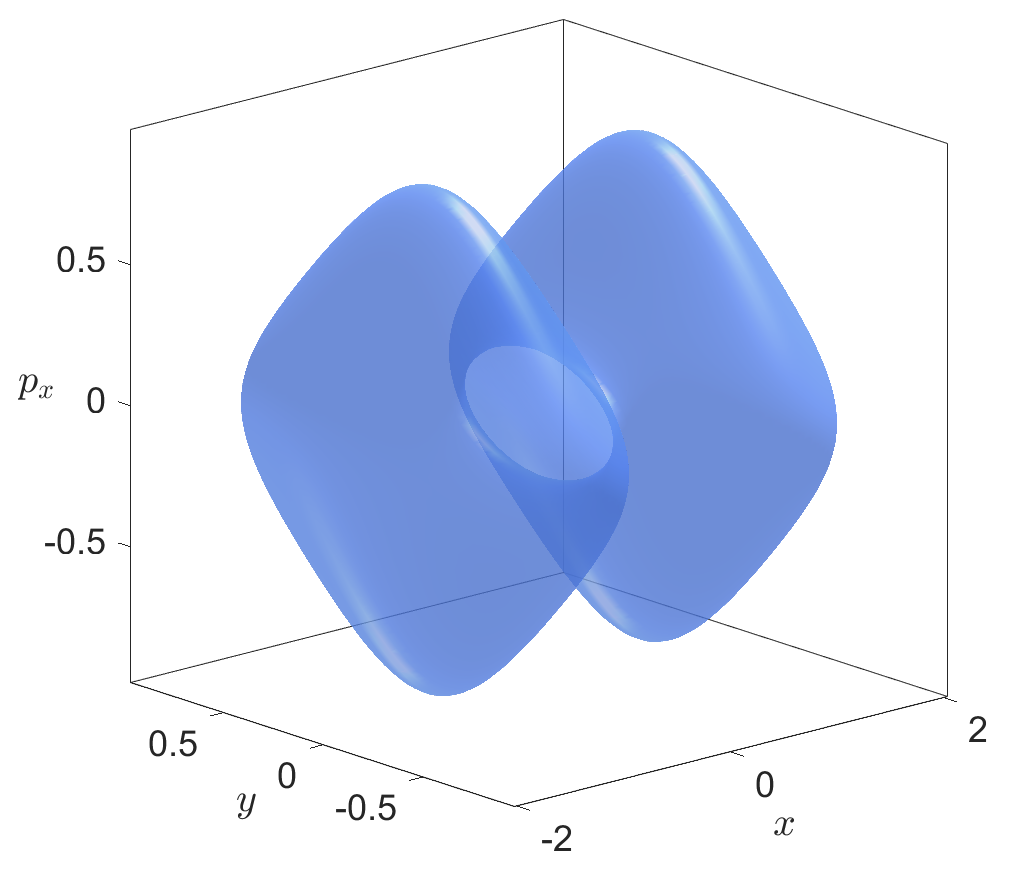
\includegraphics[scale=0.28]{energySurf_H_-01.png}
	B)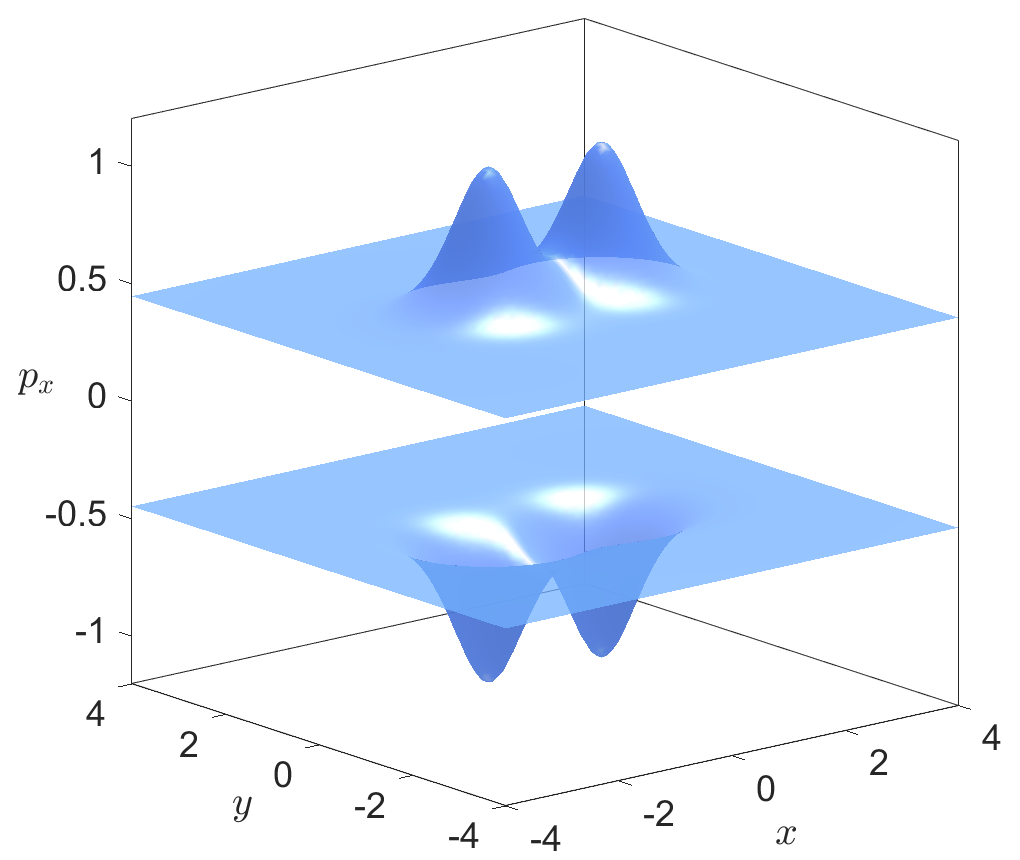
\includegraphics[scale=0.28]{energySurf_H_01.png}
	\caption{$W_0 = 1/2$ and $k = 1$. A) $H_0 = -0.1$; B) $H_0 = 0.1$.}
	\label{fig:vdw-energyHyp}
\end{figure}

\begin{figure}[htbp]
	A)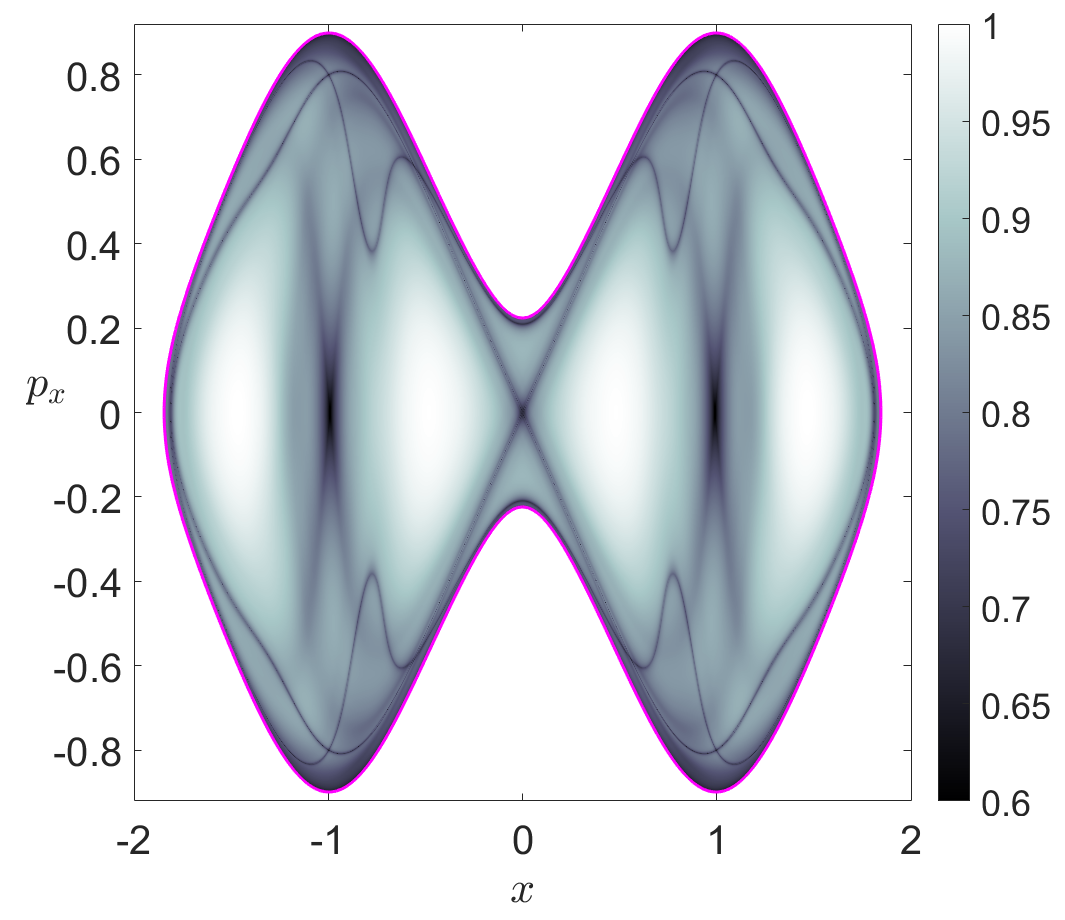
\includegraphics[scale=0.28]{H_-01_LD_tau_12_y_0.png}
	B)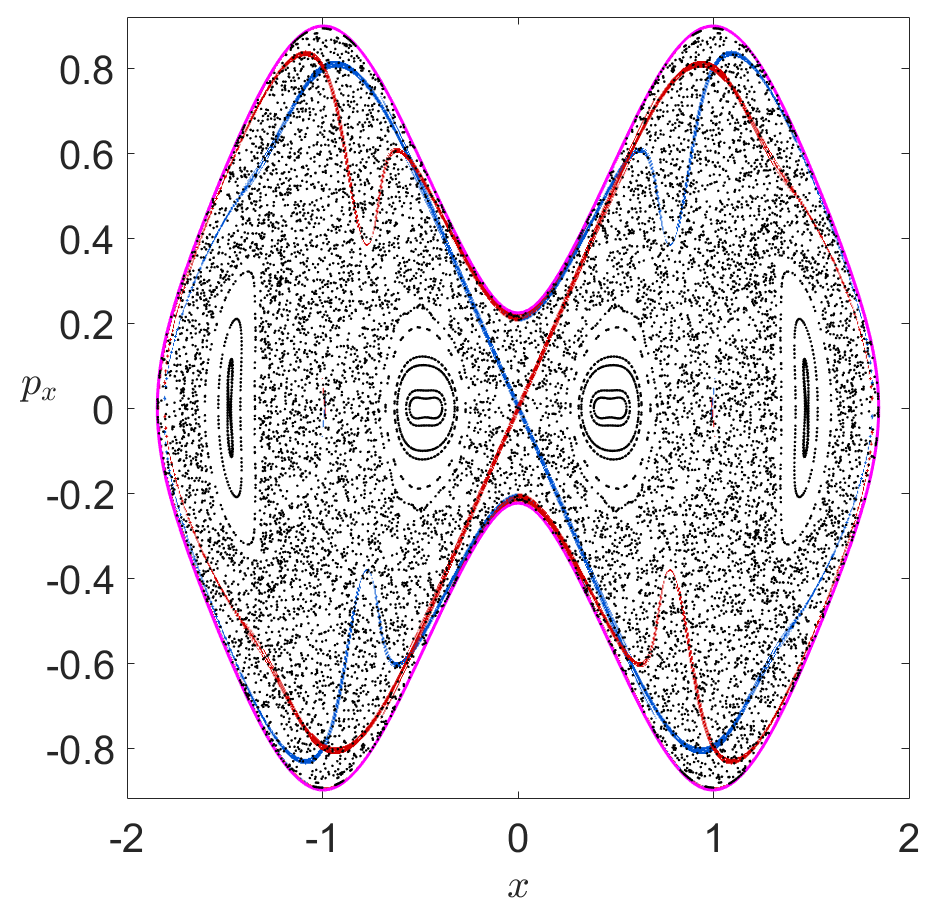
\includegraphics[scale=0.28]{H_-01_mani_tau_12_y_0.png}	
	C)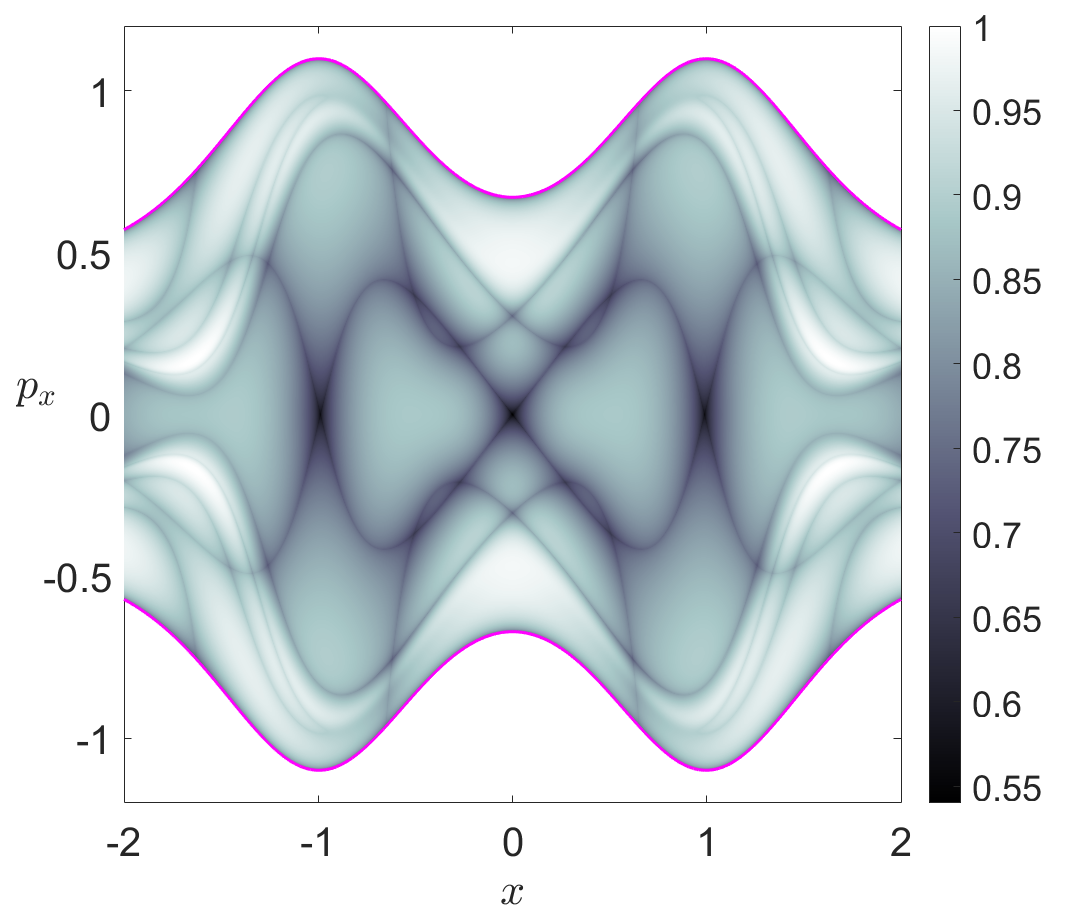
\includegraphics[scale=0.28]{H_01_LD_tau_12_y_0.png}
	D)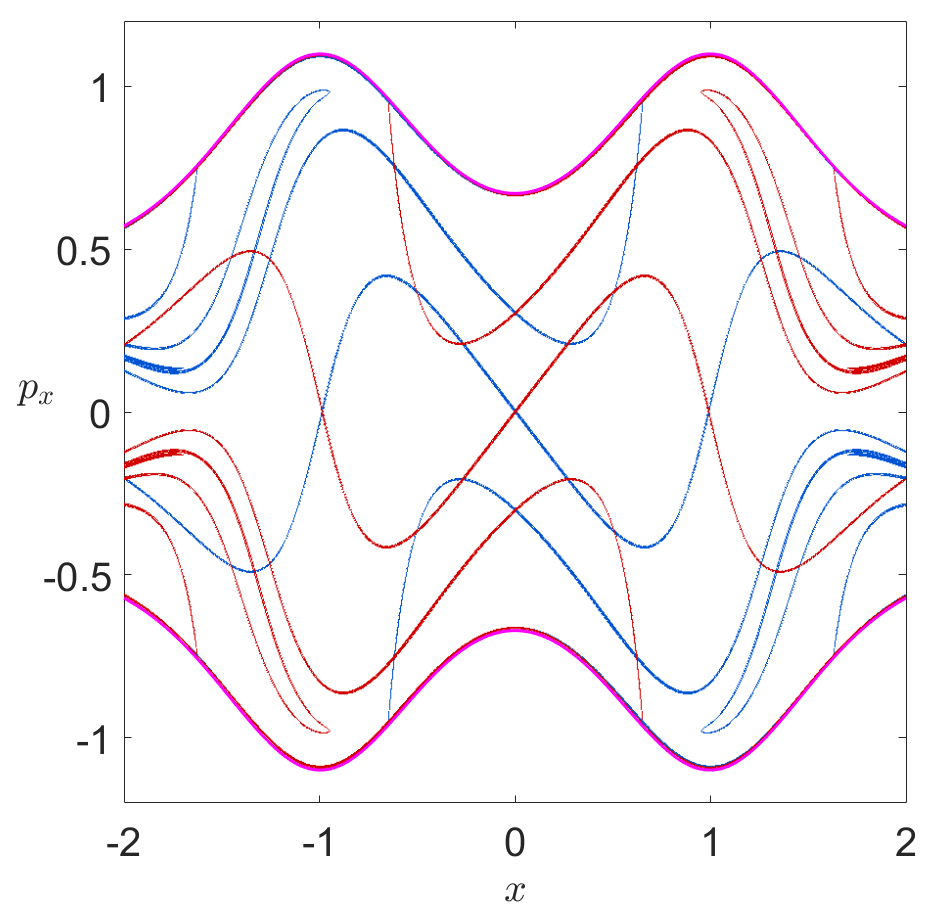
\includegraphics[scale=0.28]{H_01_mani_tau_12_y_0.png}
	\caption{Parameters $W_0 = 1/2$ and $k = 1$. Poincar\'e section $y = 0$. Top row energy $H_0 = -0.1$. Bottom row energy $H_0 = 0.1$.}
	\label{fig:ld_mani_y_0}
\end{figure}

\begin{figure}[htbp]
	A)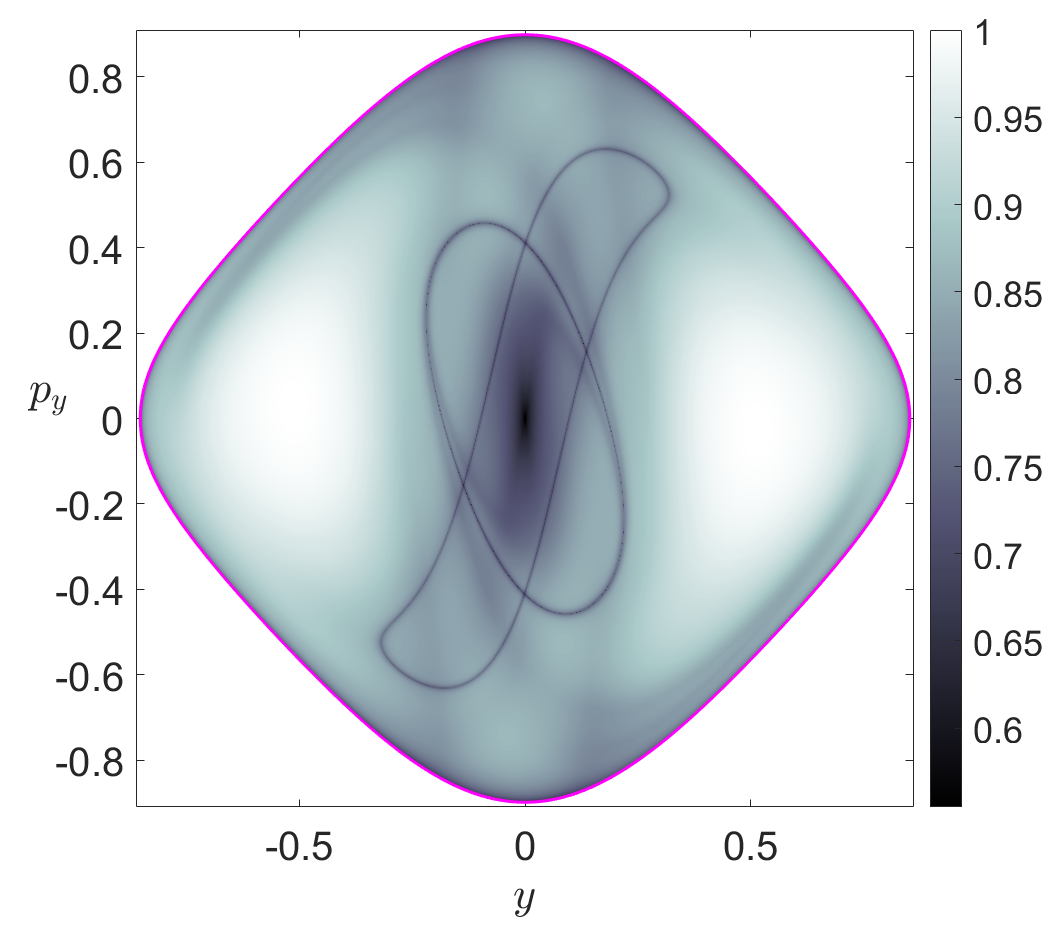
\includegraphics[scale=0.28]{H_-01_LD_tau_12_x_1.png}
	B)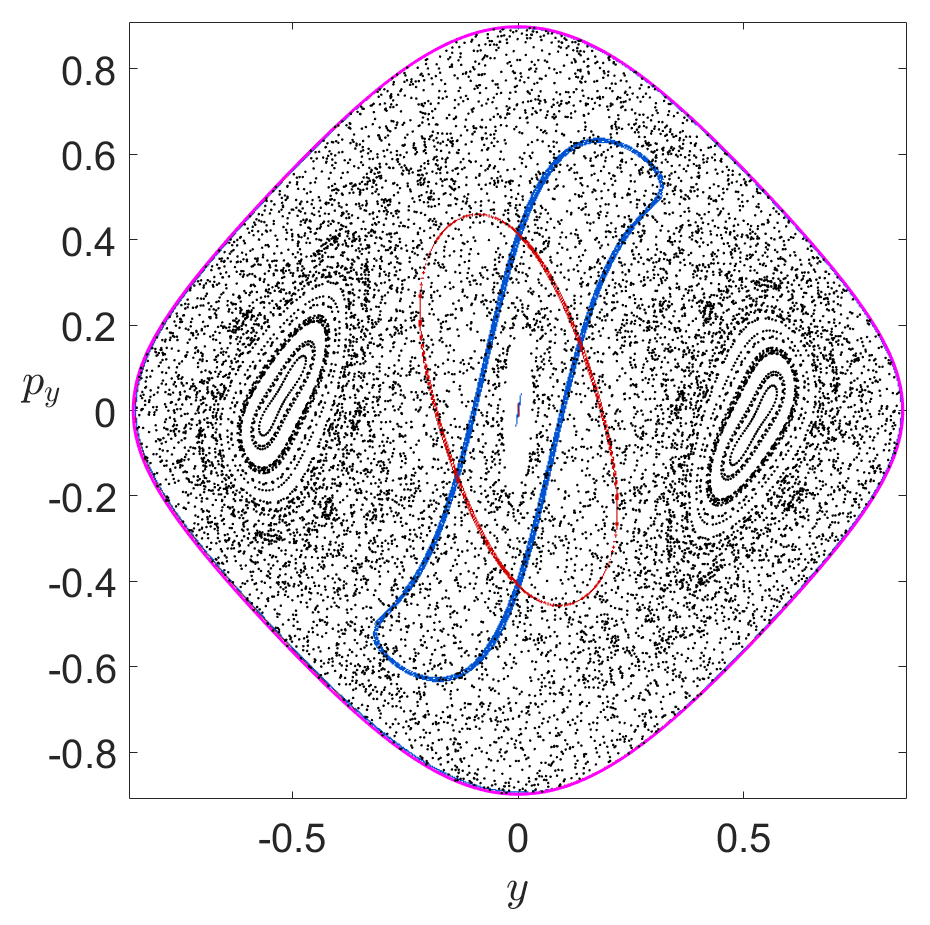
\includegraphics[scale=0.28]{H_-01_mani_tau_12_x_1.png}	
	C)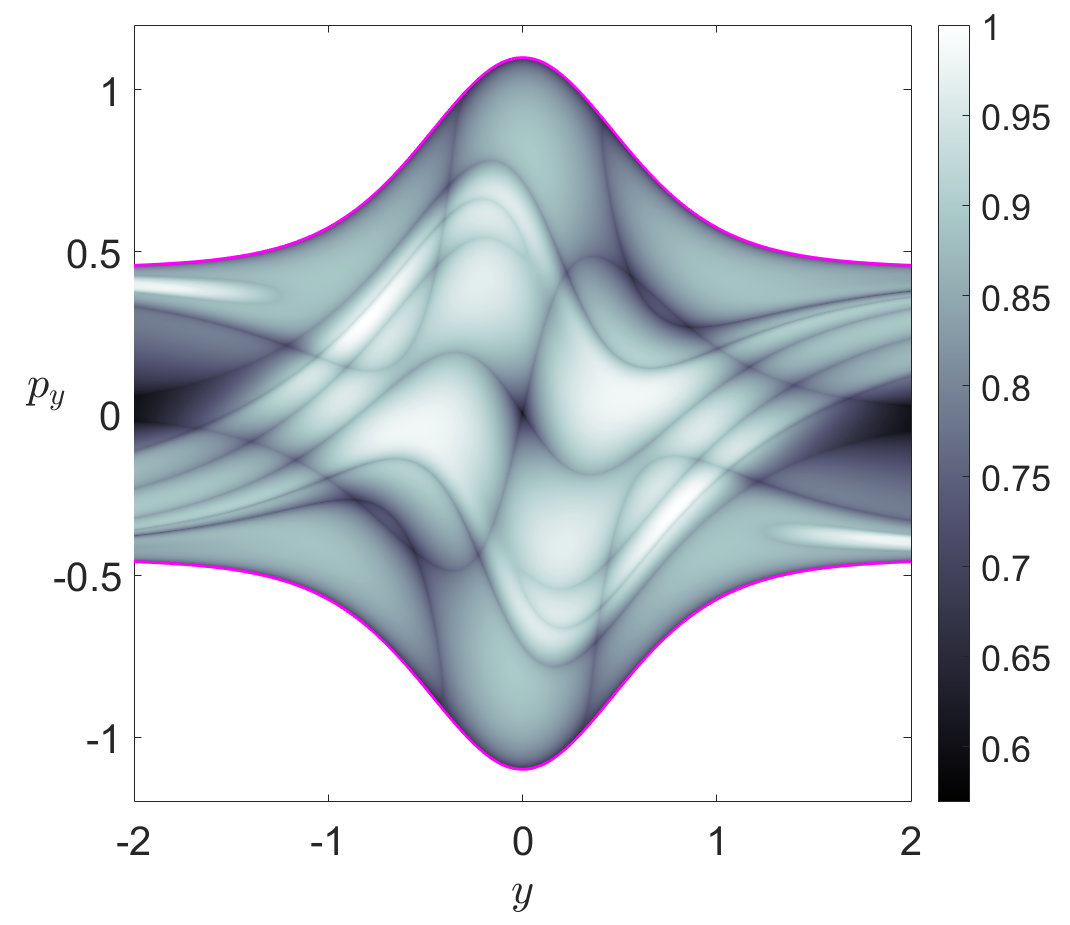
\includegraphics[scale=0.28]{H_01_LD_tau_12_x_1.png}
	D)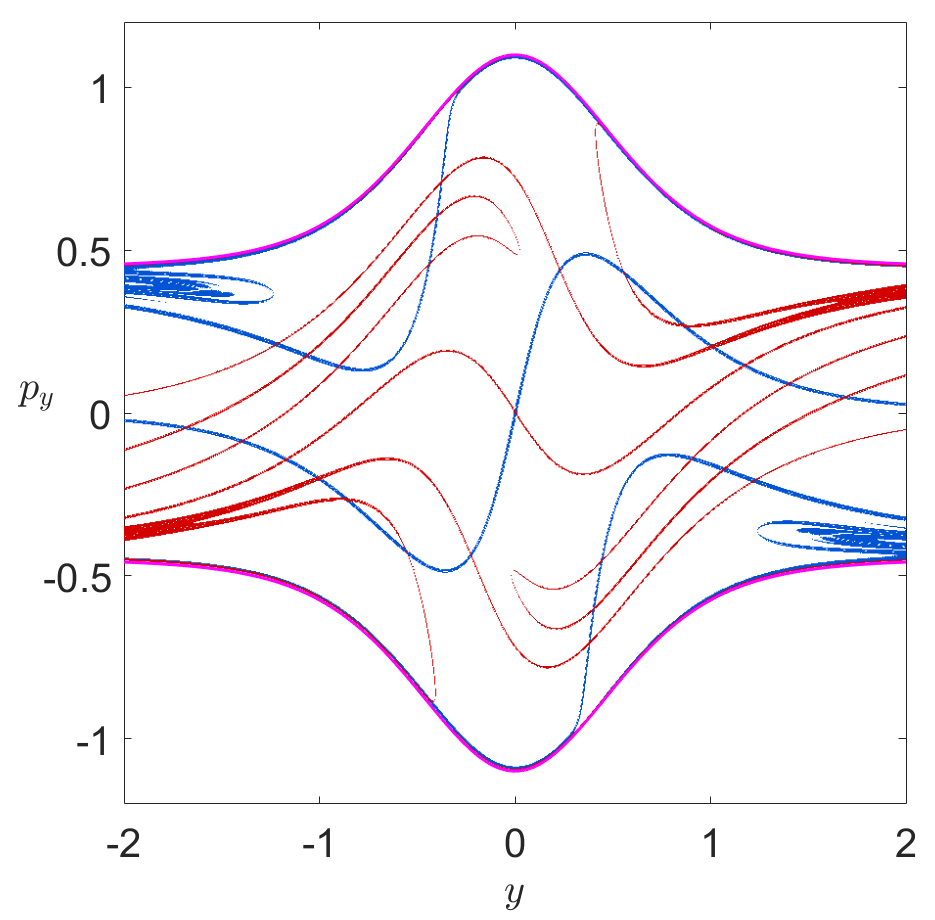
\includegraphics[scale=0.28]{H_01_mani_tau_12_x_1.png}
	\caption{Parameters $W_0 = 1/2$ and $k = 1$. Poincar\'e section $x = 1$. Top row energy $H_0 = -0.1$. Bottom row energy $H_0 = 0.1$.}
	\label{fig:ld_mani_x_1}
\end{figure}

\begin{figure}[htbp]
	A)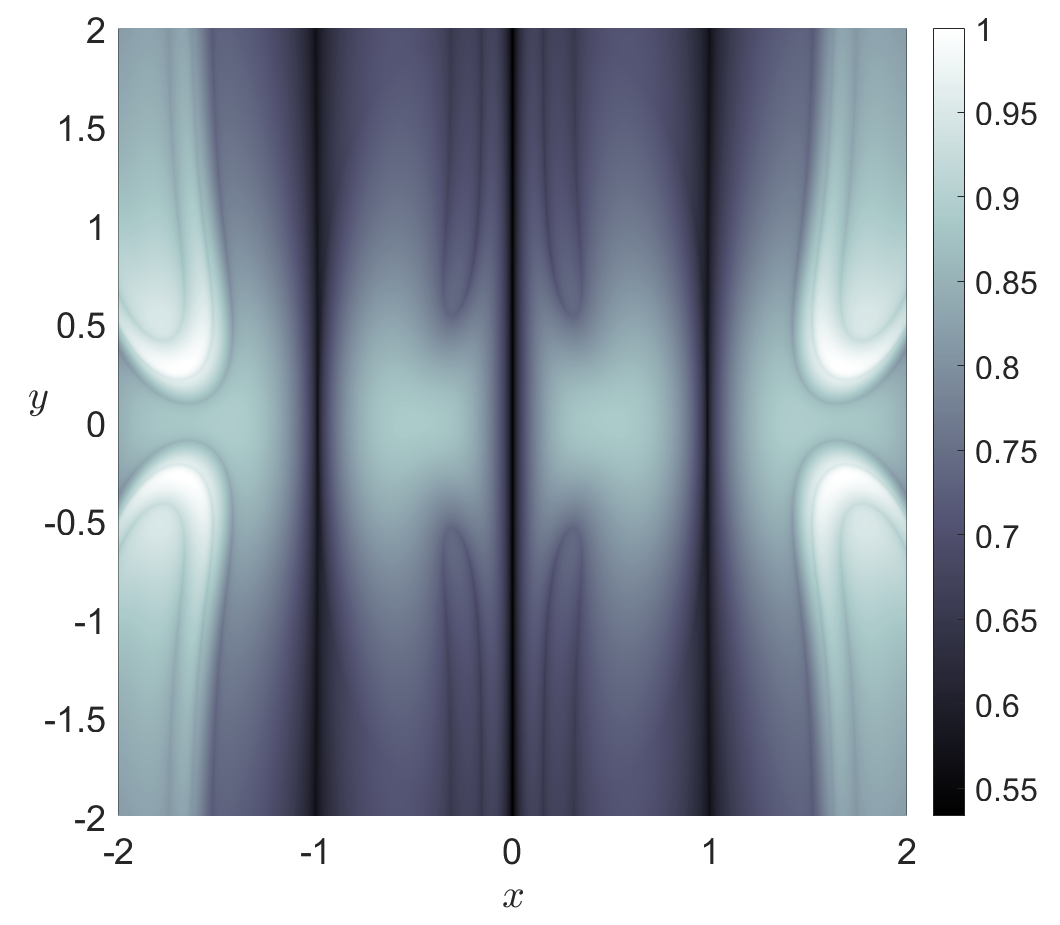
\includegraphics[scale=0.28]{H_01_LD_tau_12_px_0.png}
	B)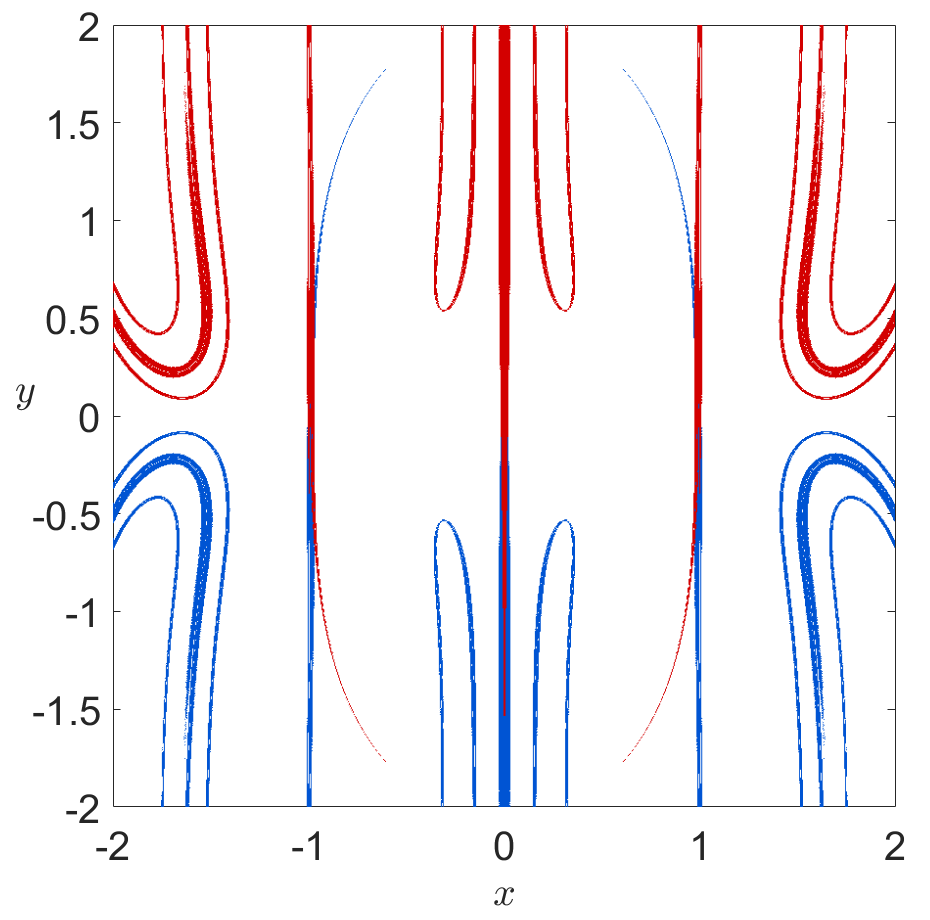
\includegraphics[scale=0.28]{H_01_mani_tau_12_px_0.png}	
	\caption{Parameters $W_0 = 1/2$ and $k = 1$. Poincar\'e section $p_x = 0$. Energy $H_0 = 0.1$.}
	\label{fig:ld_mani_px_0}
\end{figure}


\begin{figure}[htbp]
	A)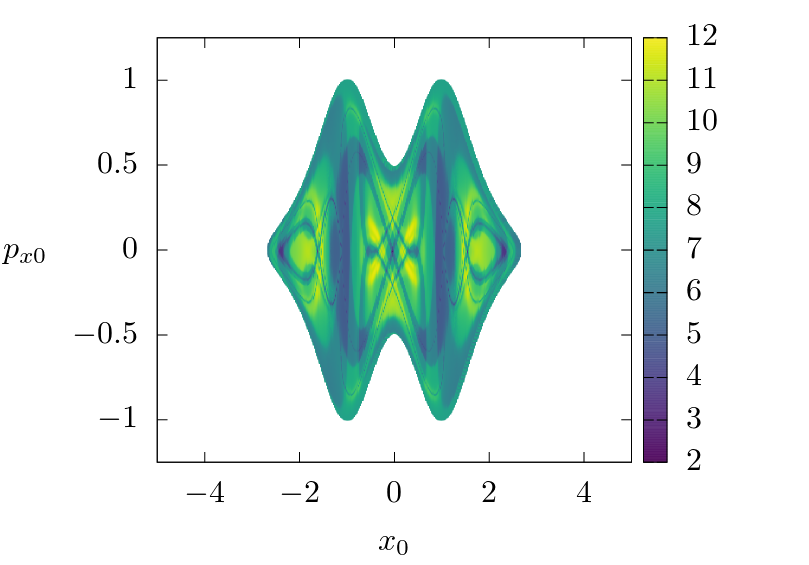
\includegraphics[scale=0.35]{ld_xpx_t20_E-001.png}
	B)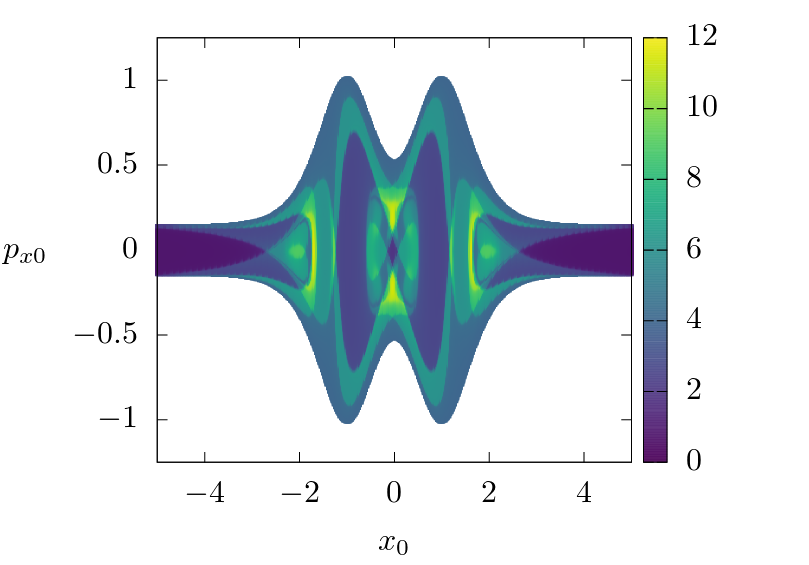
\includegraphics[scale=0.35]{ld_xpx_t20_E001.png}	
	\caption{Parameters $W_0 = 1/2$ and $k = 1$. Surface $y = 0$. $H_0 =-0.01, 0.01$.  }
	\label{fig:ld_x_px}
\end{figure}

\begin{figure}[htbp]
	A)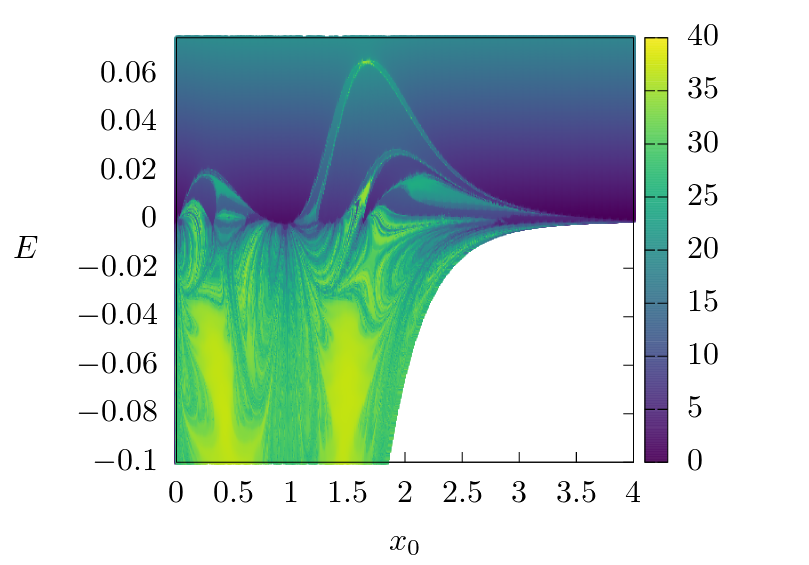
\includegraphics[scale=0.35]{ld_t60_line_x_E.png}
	B)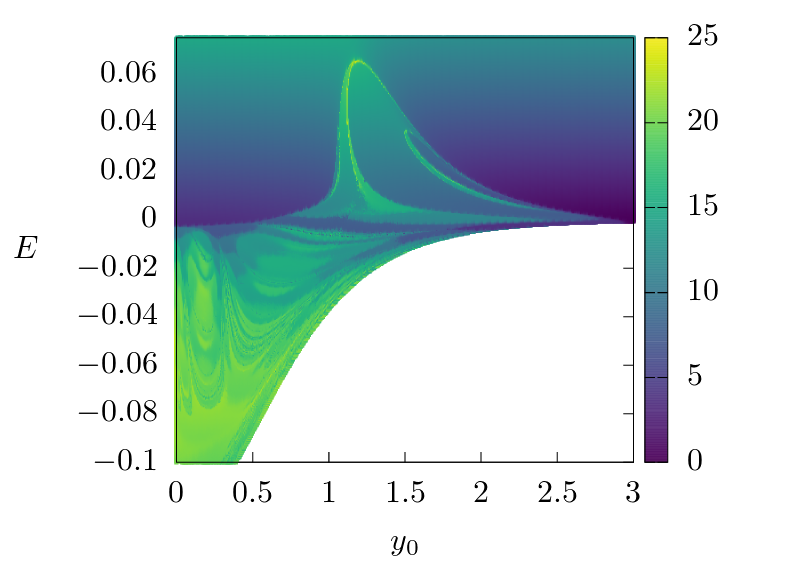
\includegraphics[scale=0.35]{ld_t60_line_y_E.png}
	\caption{ Bifurcations diagrams based on Lagrangian descriptor $E$ vs $x_0$ and $E$ vs $y_0$.  Parameters $W_0 = 1/2$ and $k = 1$. }
	\label{fig:ld_E_xy}
\end{figure}

\begin{figure}[htbp]
	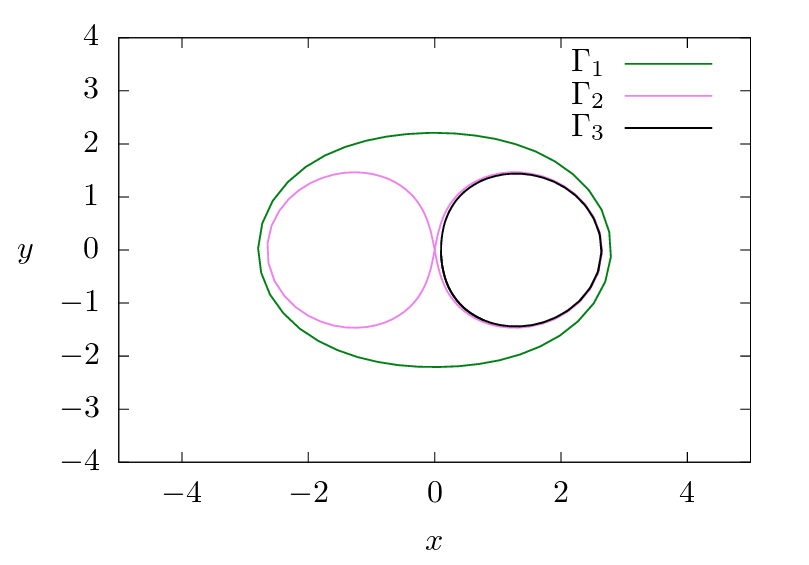
\includegraphics[scale=0.5]{orbits_2D.png}
	\caption{Periodic orbits in the configuration space. $E$ = 0.01. }
	\label{fig:ld_E_xy}
\end{figure}

In this section we will study the transport associated with the roaming phenomenon. Let's consider the trajectories that go from one potential well to the other potential well and the trajectories that go from one potential well to the asymptotic. To carry out this study let's consider 3 regions in the configuration space: 2 circles with the same radius, whose centres are in the minimum of each potential well, regions A and B, and a circle containing the two potential wells where the trajectories are opposite in origin and whose border is in the asymptotic region, region C. In the next numerical example, the radios to define the regions A,B, and C are 1.5 and 5.0 respectively.


\begin{figure}[htbp]
	A)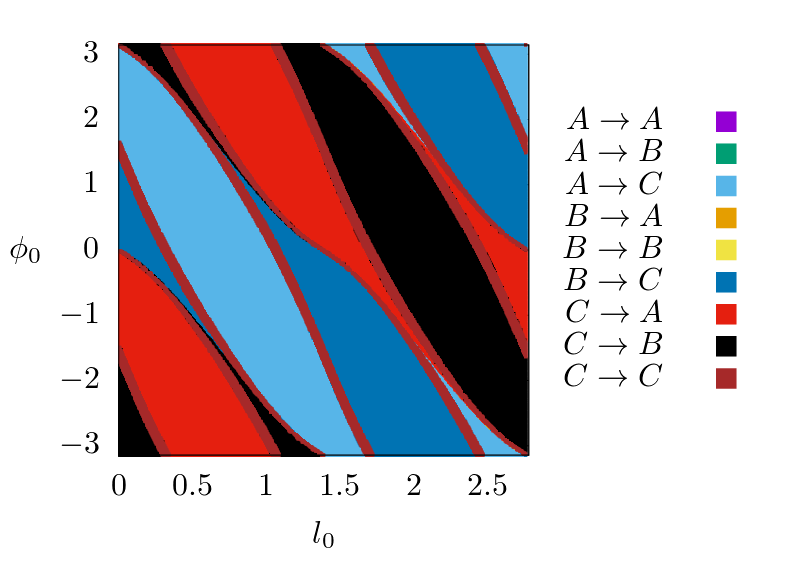
\includegraphics[scale=0.35]{fate_map_ds_gamma1E_001.png}
	B)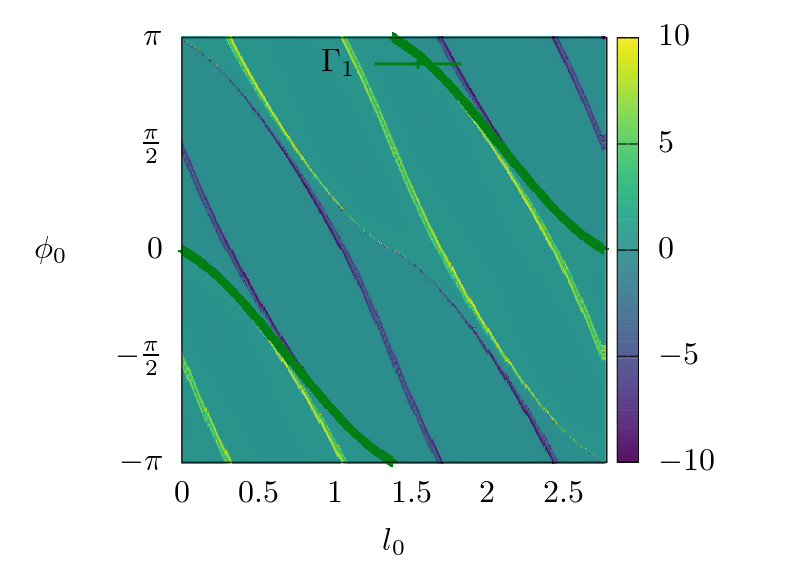
\includegraphics[scale=0.35]{ld_action_ds_gamma1_E_001.png}
	C)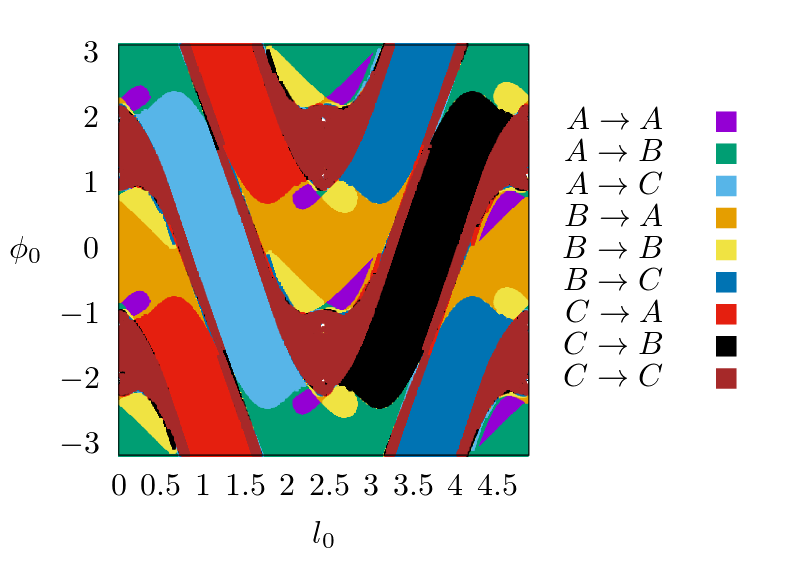
\includegraphics[scale=0.35]{fate_map_ds_gamma2E_001.png}
	D)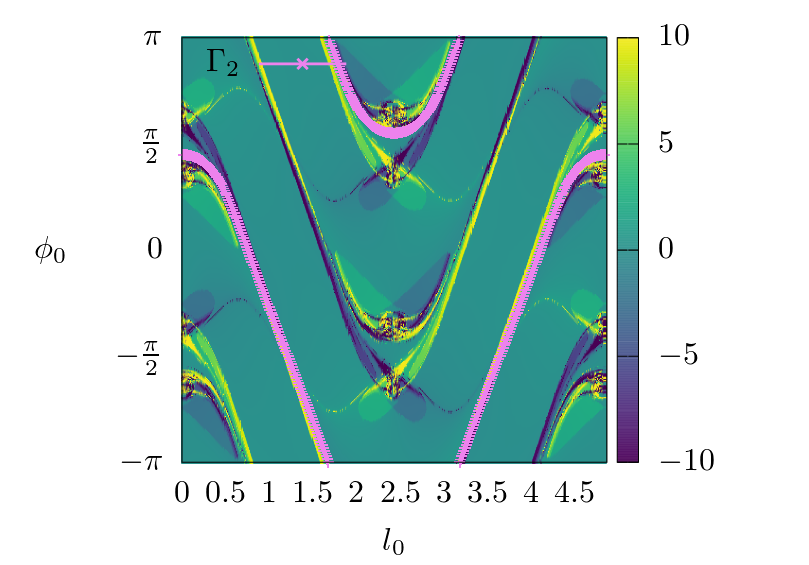
\includegraphics[scale=0.35]{ld_action_ds_gamma2_E_001.png}
	E)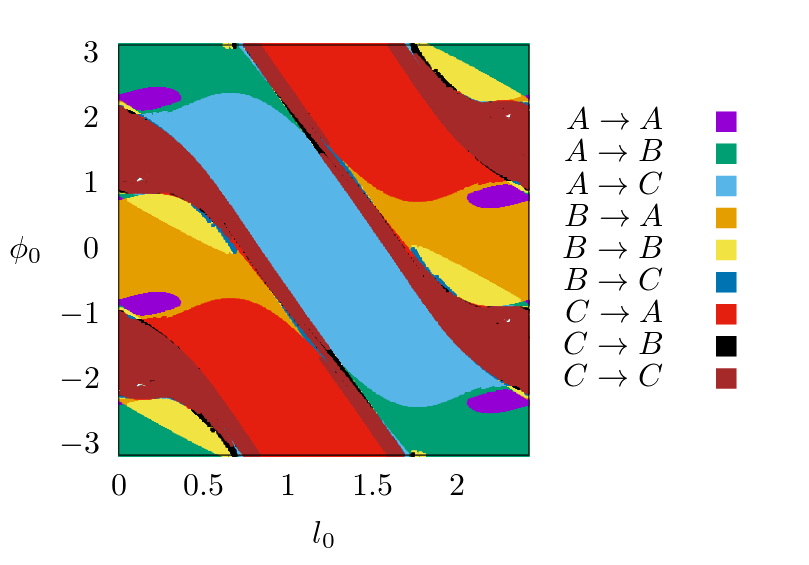
\includegraphics[scale=0.35]{fate_map_ds_gamma3E_001.png}
	F)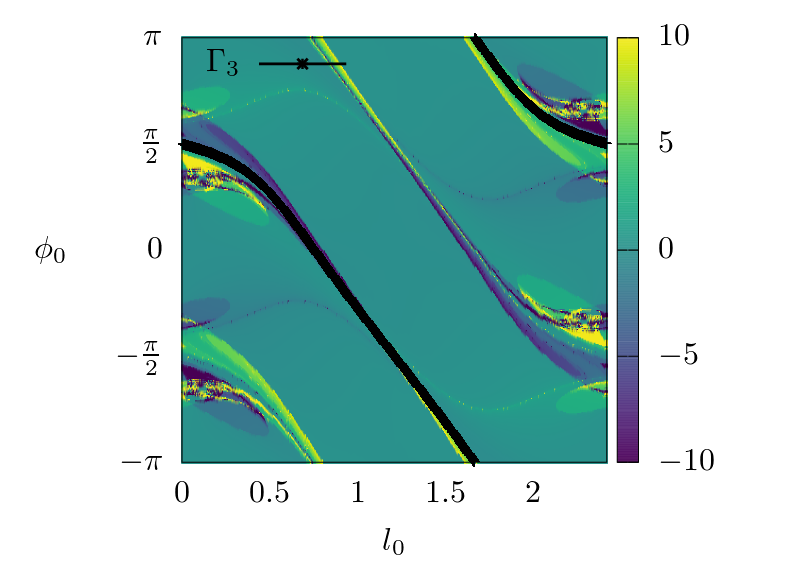
\includegraphics[scale=0.35]{ld_action_ds_gamma3_E_001.png}
	\caption{ Fate maps and Lagrangian descriptors evaluated on the dividing surface corresponding to periodic orbits $\Gamma_1$, $\Gamma_2$, and $\Gamma_3$ ($E$ =0.01). }
	\label{fig:ld_fm_ds}
\end{figure}


\begin{figure}[htbp]
	A)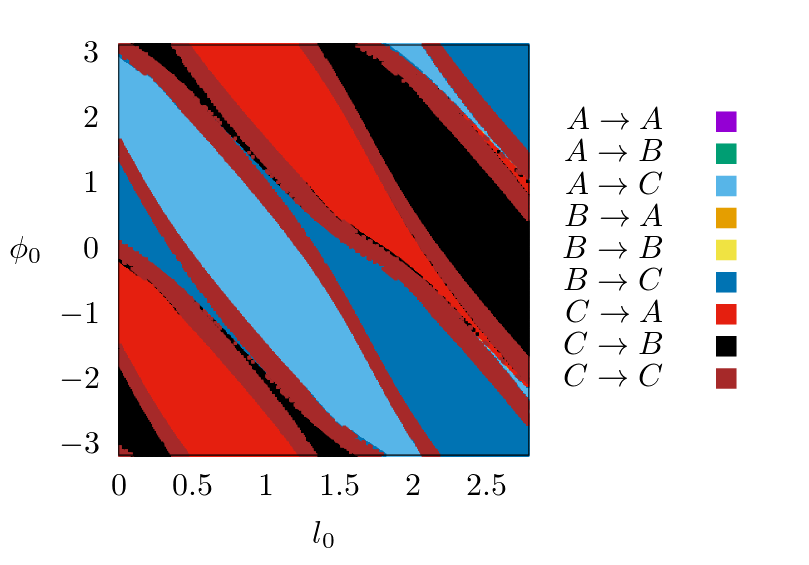
\includegraphics[scale=0.35]{fate_map_ds_gamma1E_0019.png}
	B)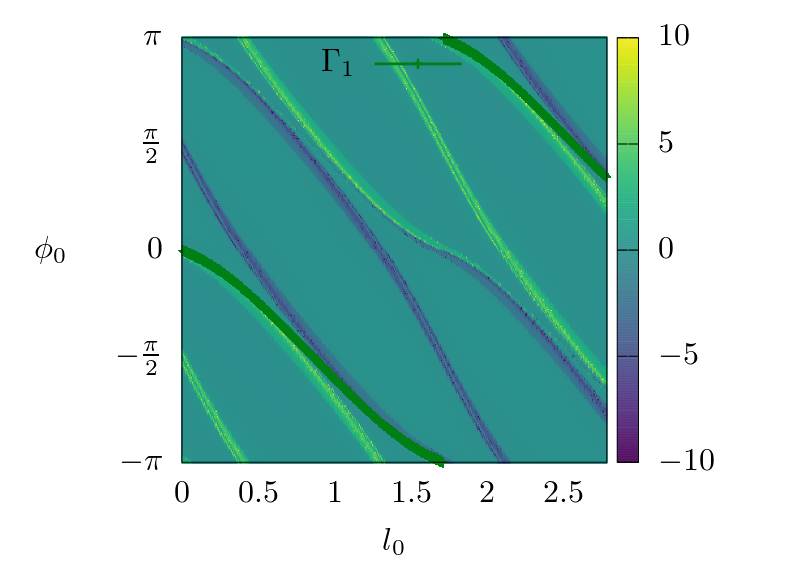
\includegraphics[scale=0.35]{ld_action_ds_gamma1_E_0019.png}
	C)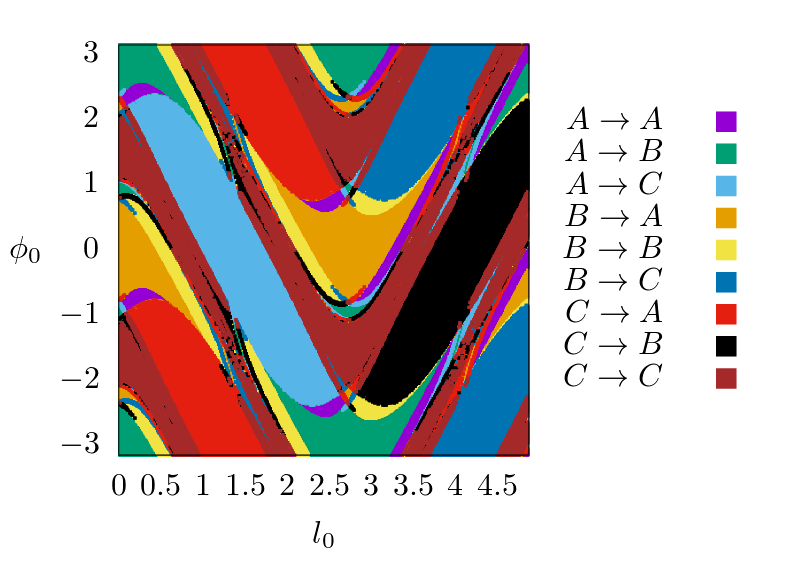
\includegraphics[scale=0.35]{fate_map_ds_gamma2E_0019.png}
	D)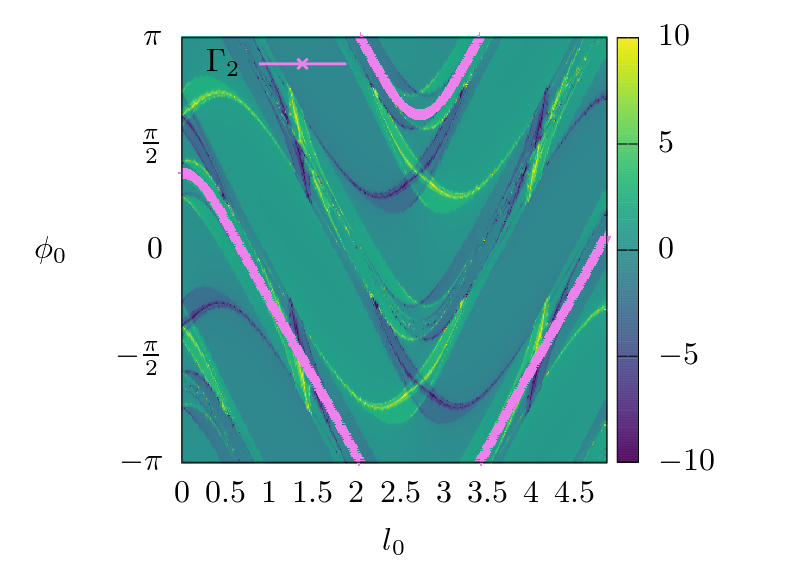
\includegraphics[scale=0.35]{ld_action_ds_gamma2_E_0019.png}
	E)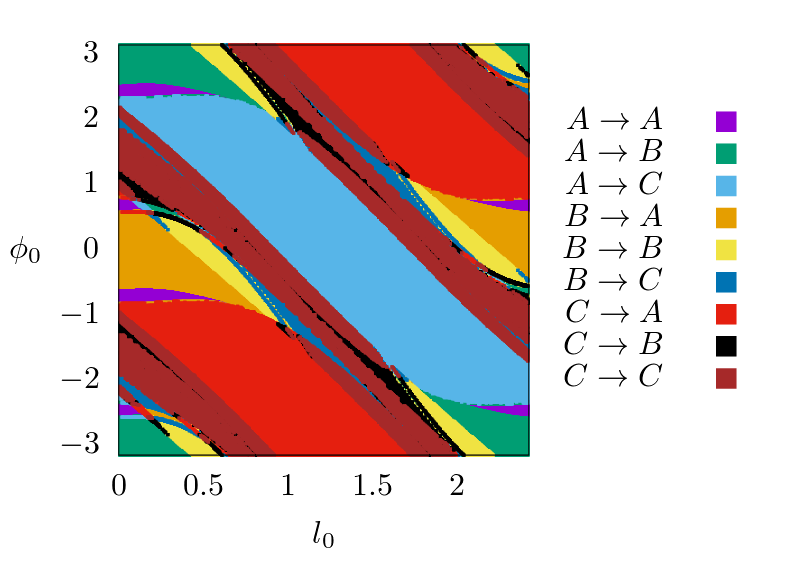
\includegraphics[scale=0.35]{fate_map_ds_gamma3E_0019.png}
	F)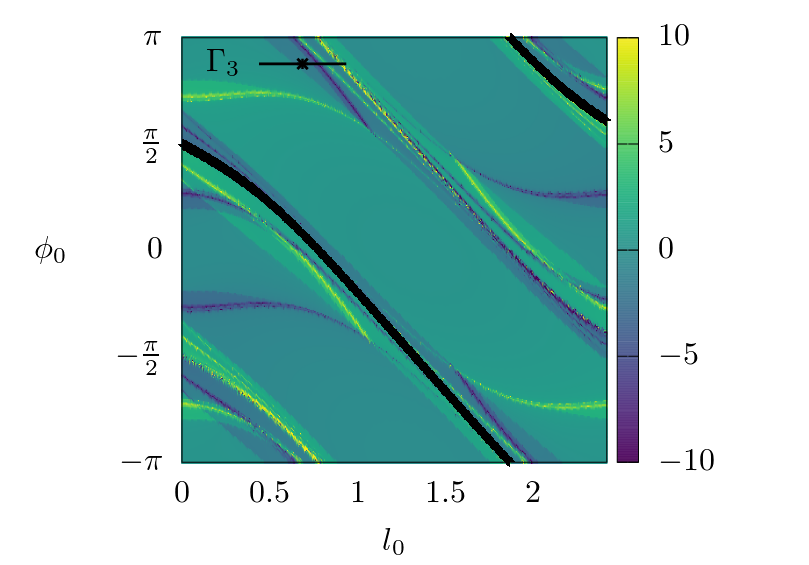
\includegraphics[scale=0.35]{ld_action_ds_gamma3_E_0019.png}
	\caption{ Fate maps and Lagrangian descriptors evaluated on the dividing surface corresponding to periodic orbits $\Gamma_1$, $\Gamma_2$, and $\Gamma_3$ ($E$ =0.019, before bifurcation of $\Gamma_3$). }
	\label{fig:ld_fm_ds}
\end{figure}


\begin{figure}[htbp]
	A)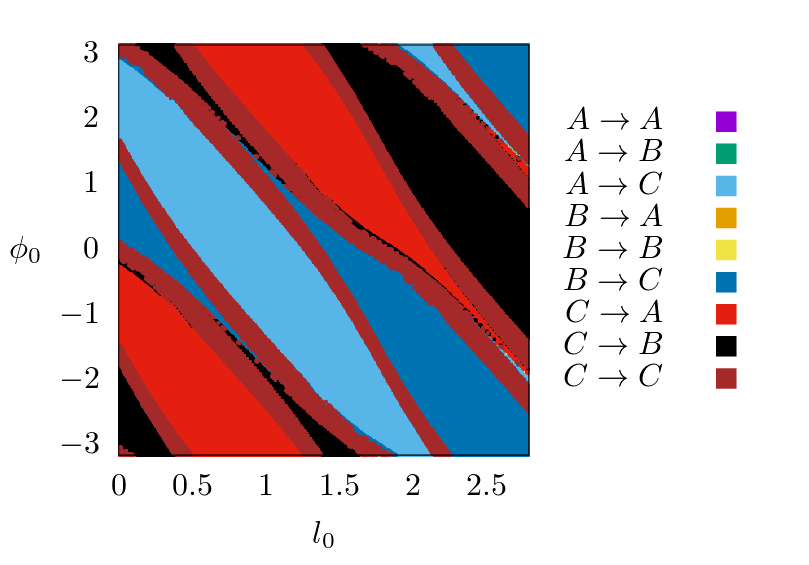
\includegraphics[scale=0.35]{fate_map_ds_gamma1E_0021.png}
	B)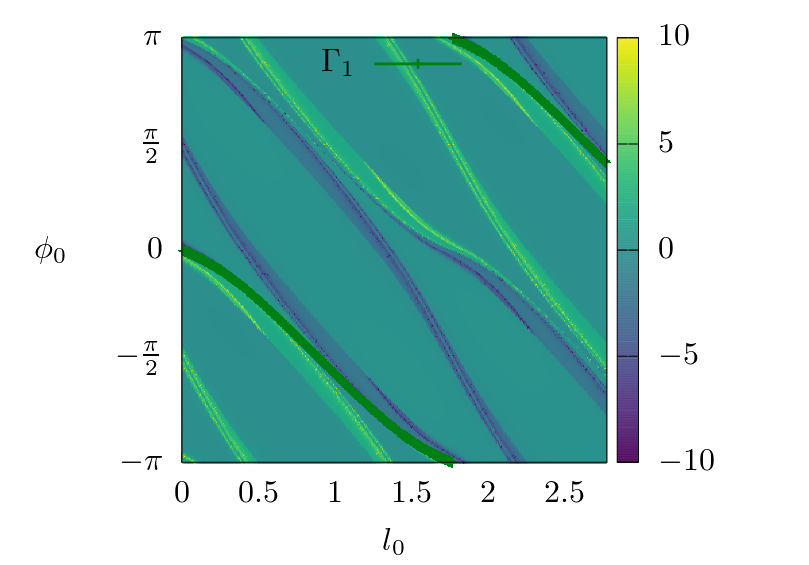
\includegraphics[scale=0.35]{ld_action_ds_gamma1_E_0021.png}
	C)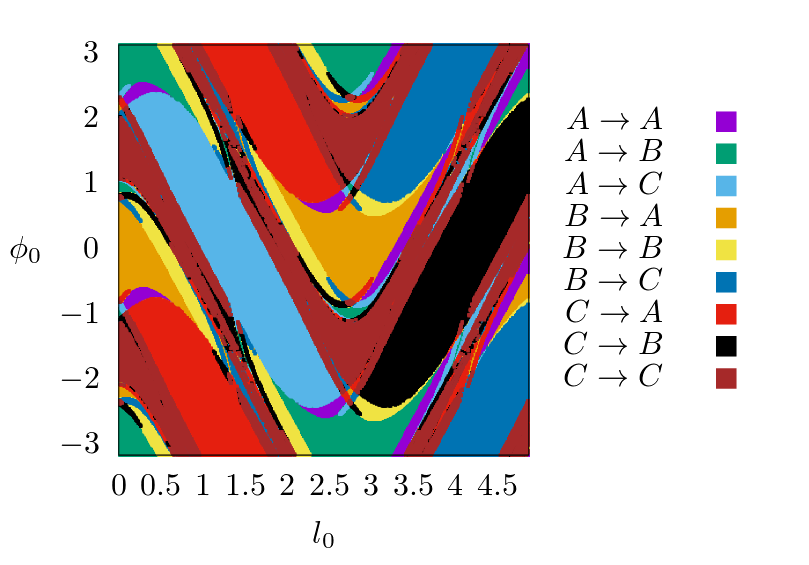
\includegraphics[scale=0.35]{fate_map_ds_gamma2E_0021.png}
	D)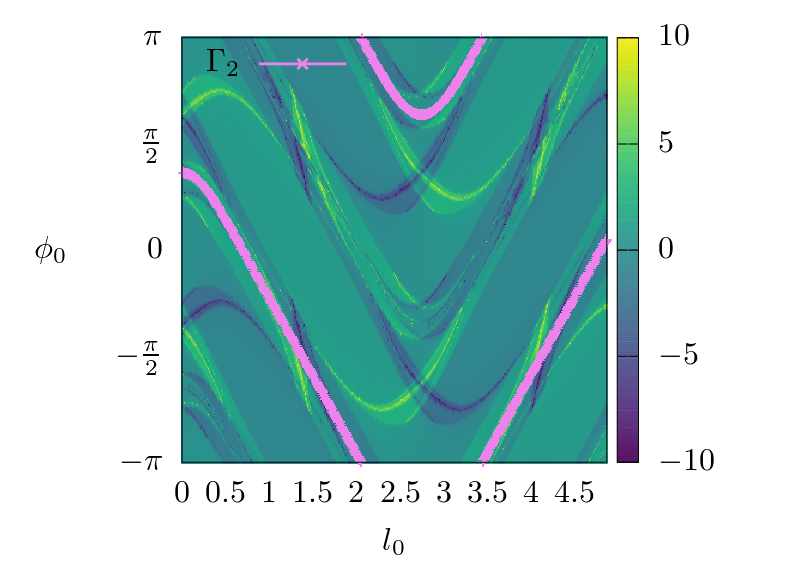
\includegraphics[scale=0.35]{ld_action_ds_gamma2_E_0021.png}
	\caption{ Fate maps and Lagrangian descriptors evaluated on the dividing surface corresponding to periodic orbits $\Gamma_1$ and $\Gamma_2$ ($E$ =0.021, after bifurcation of $\Gamma_3$). }
	\label{fig:ld_fm_ds}
\end{figure}


\begin{figure}[htbp]
	A)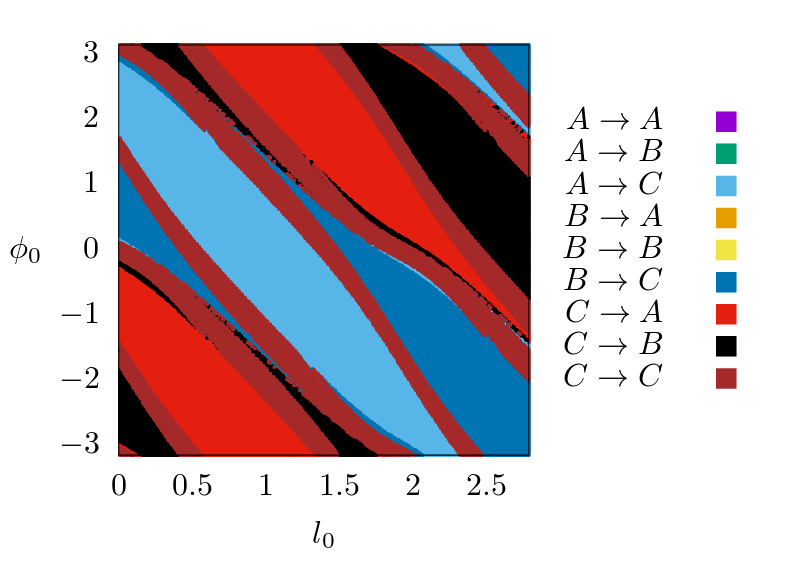
\includegraphics[scale=0.35]{fate_map_ds_gamma1E_0027.png}
	B)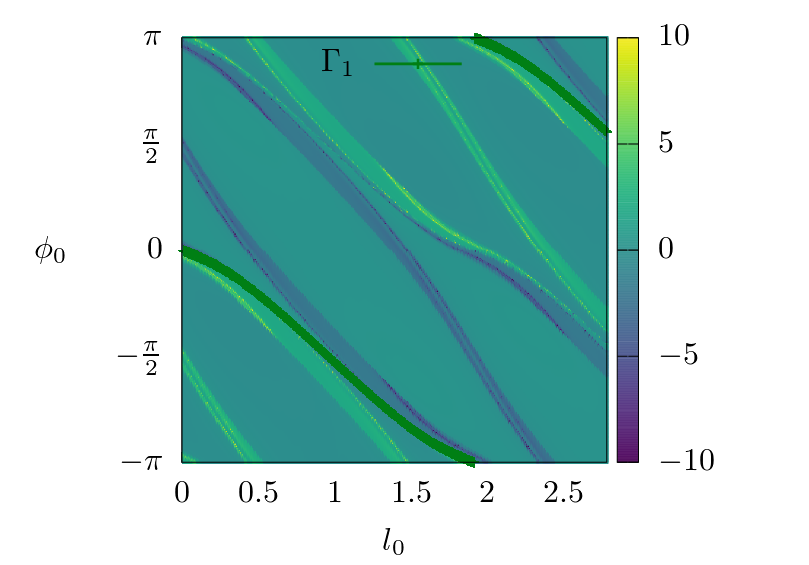
\includegraphics[scale=0.35]{ld_action_ds_gamma1_E_0027.png}
	C)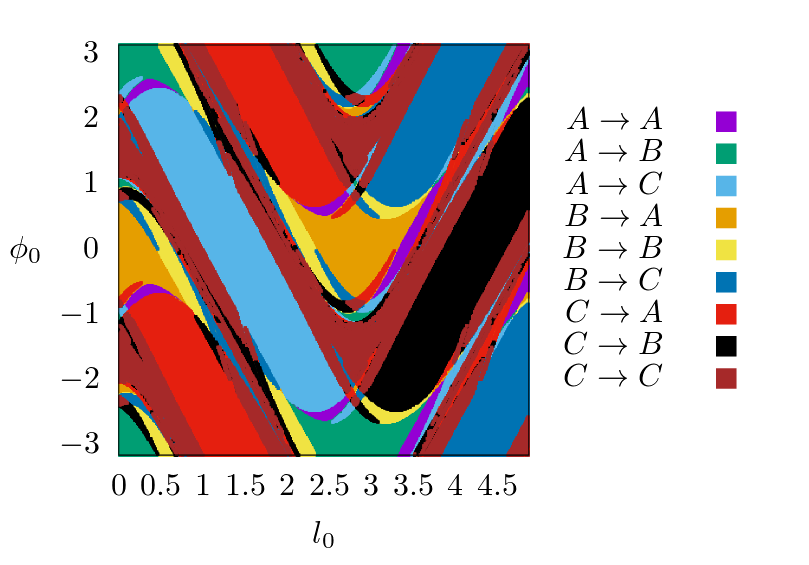
\includegraphics[scale=0.35]{fate_map_ds_gamma2E_0027.png}
	D)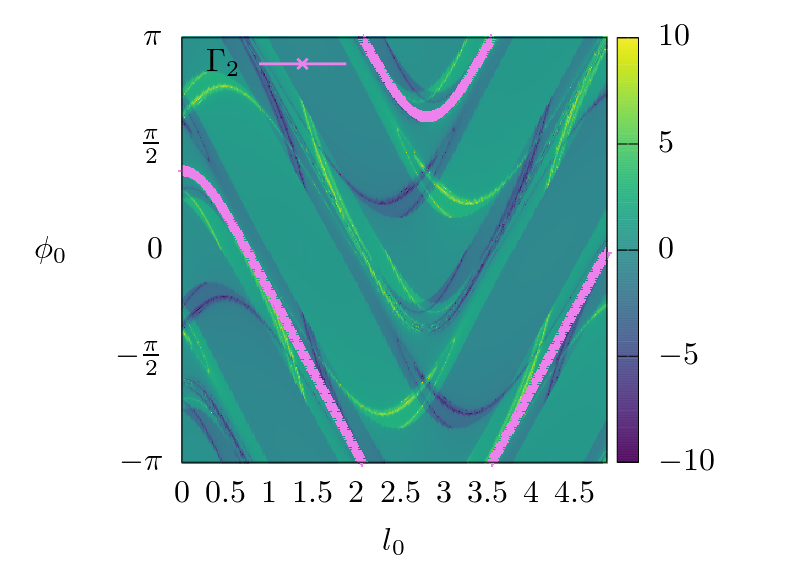
\includegraphics[scale=0.35]{ld_action_ds_gamma2_E_0027.png}
	\caption{ Fate maps and Lagrangian descriptors evaluated on the dividing surface corresponding to periodic orbits $\Gamma_1$ and $\Gamma_2$ ($E$ =0.027, before bifurcation of $\Gamma_2$  ). }
	\label{fig:ld_fm_ds}
\end{figure}


\begin{figure}[htbp]
	A)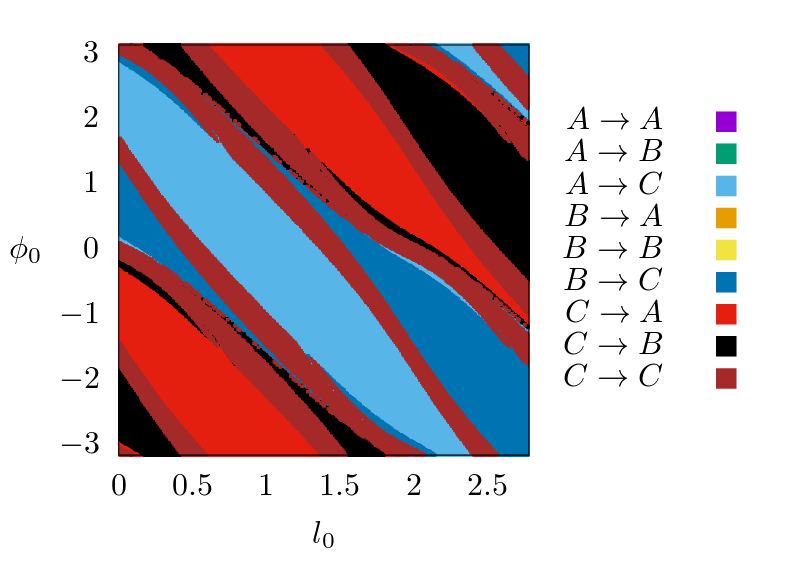
\includegraphics[scale=0.35]{fate_map_ds_gamma1E_003.png}
	B)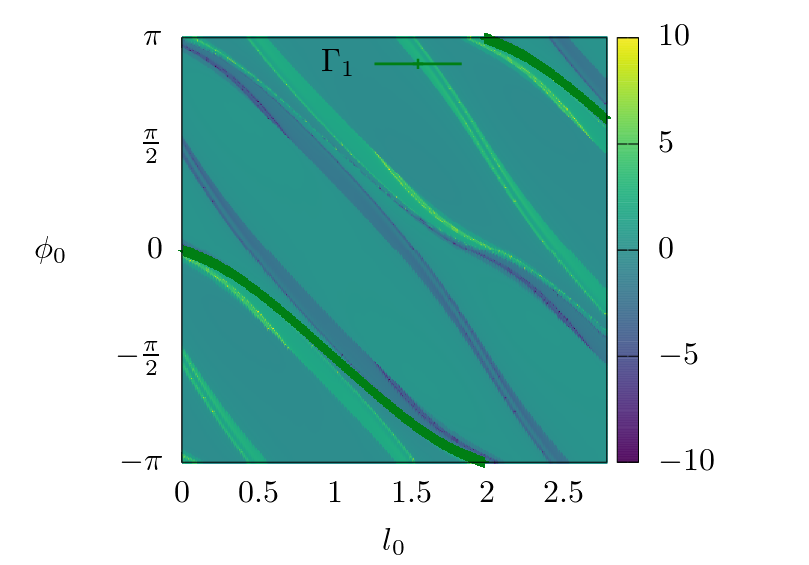
\includegraphics[scale=0.35]{ld_action_ds_gamma1_E_003.png}
	\caption{ Fate maps and Lagrangian descriptors evaluated on the dividing surface corresponding to periodic orbits $\Gamma_1$ and $\Gamma_2$ ($E$ =0.03, after bifurcation of $\Gamma_2$  ). }
	\label{fig:ld_fm_ds}
\end{figure}



\begin{figure}[htbp]
	A)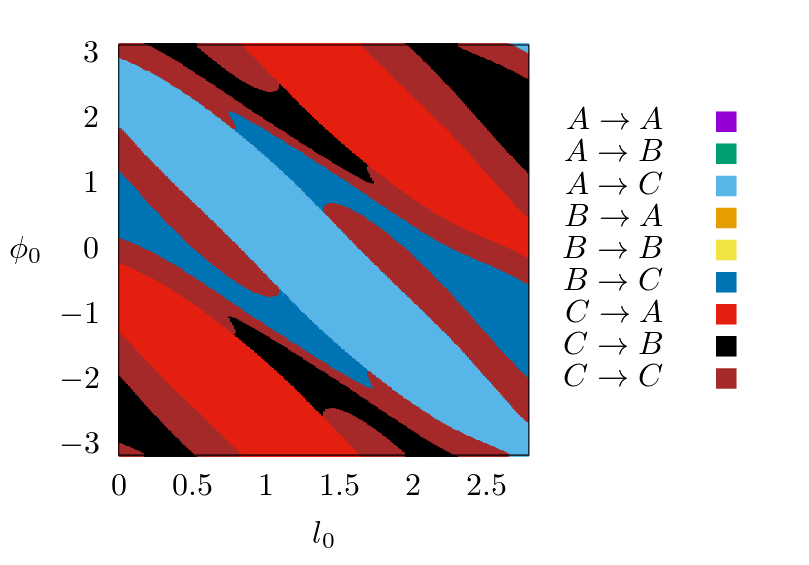
\includegraphics[scale=0.35]{fate_map_ds_gamma1E_0065.png}
	B)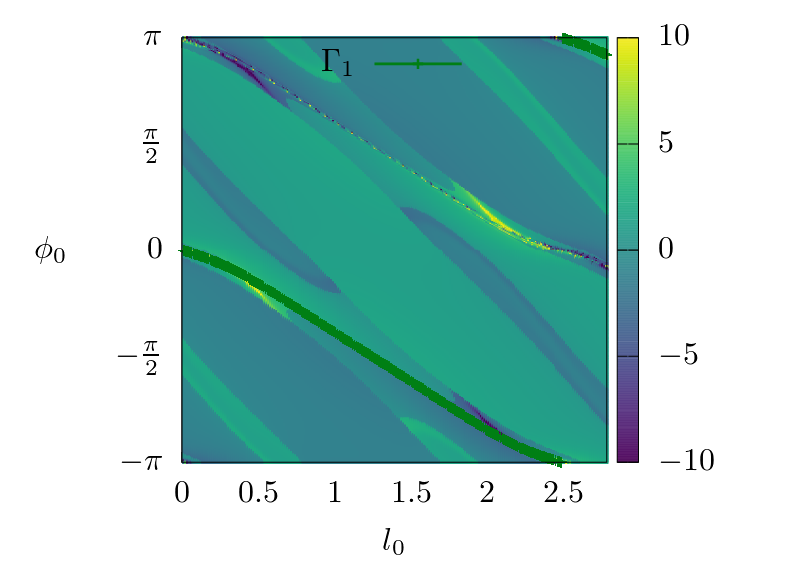
\includegraphics[scale=0.35]{ld_action_ds_gamma1_E_0065.png}
	\caption{ Fate maps and Lagrangian descriptors evaluated on the dividing surface corresponding to periodic orbit $\Gamma_1$ ($E$ =0.065, before bifurcation of $\Gamma_1$ ). }
	\label{fig:ld_fm_ds}
\end{figure}


\begin{figure}
    \centering
    A)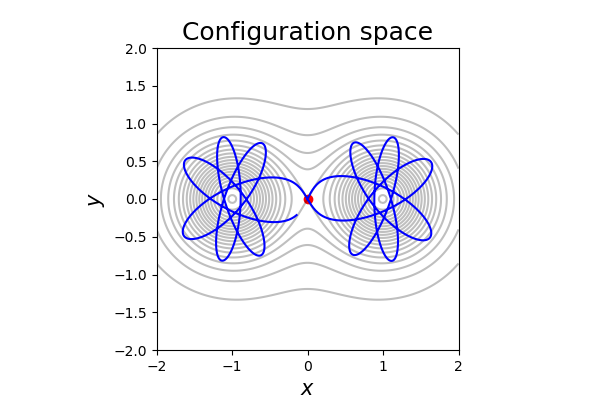
\includegraphics{traj_type2.png}
    B)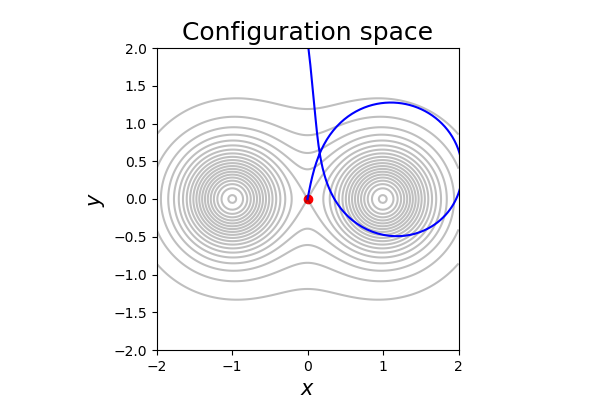
\includegraphics{traj_escapping.png}
    \caption{Example trajectories for bounding and dissociation energies, respectively. A) $E = -0.1$, B) $E=0.01$, with identical initial condition $(x_0, y_0) = (0, 0)$, and $p_{x,0} = 0.1$}
    \label{fig:my_label}
\end{figure}

%%%%%%%%%%%%%%%%%%%%%%%%%%%%%%%

\begin{figure}
    \centering
    A)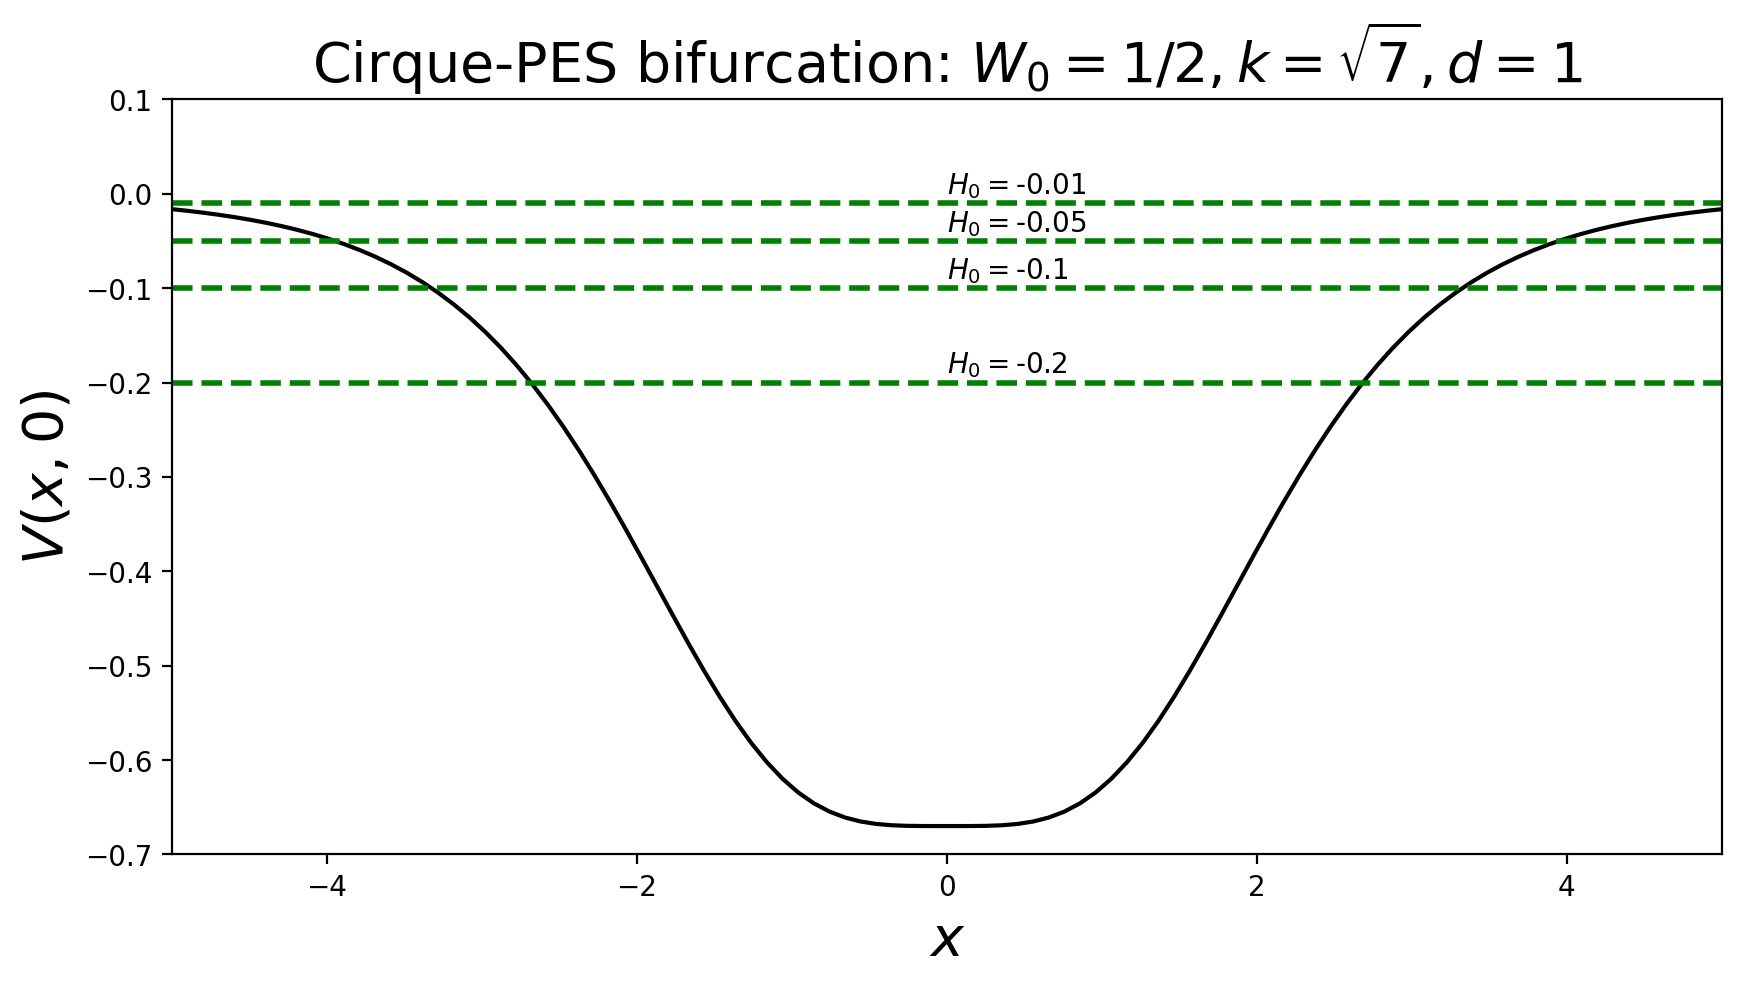
\includegraphics[width=0.45\textwidth]{pes_bifurcation_energy_levels.png}
    B)\includegraphics[width=0.45\textwidth]{pes_y_bifurcation_energy_levels.png}
    \caption{PES profile A) $y=0$; B) $x=0$; for critical bifurcation values and comparison with energy levels $H_0$}
\end{figure}

\begin{figure}[htbp]
	A)\includegraphics[scale=0.3]{PS_cirque_H_-0_2_y_0_w0_1div2_d_1_k_sqrt7.png}
	B)\includegraphics[scale=0.3]{PS_cirque_H_-0_1_y_0_w0_1div2_d_1_k_sqrt7.png}	
	C)\includegraphics[scale=0.3]{PS_cirque_H_-0_05_y_0_w0_1div2_d_1_k_sqrt7.png}
	D)\includegraphics[scale=0.3]{PS_cirque_H_-0_01_y_0_w0_1div2_d_1_k_sqrt7.png}
	\caption{Poincar\'e section $y = 0$ for the model parameters $W_0 = 1/2$, $k = \sqrt{7}$ and $d = 1$. The energy of the system is: A) $H_0 = -0.2$; B) $H_0 = -0.1$ ; C) $H_0 = -0.05$; D) $H_0 = -0.01$.}
	\label{fig:psec_y_0_bif}
\end{figure}

\begin{figure}
    \centering
    A) $H_0 = -0.2$ \includegraphics[width=0.6\textwidth]{LD_H0_-0_2_x-px_PES_bifurcation.png}\\
    A) $H_0 = -0.1$ \includegraphics[width=0.6\textwidth]{LD_H0_-0_1_x-px_PES_bifurcation.png}\\
    A) $H_0 = -0.05$ \includegraphics[width=0.6\textwidth]{LD_H0_-0_05_x-px_PES_bifurcation.png}\\
    A) $H_0 = -0.01$ \includegraphics[width=0.6\textwidth]{LD_H0_-0_01_x-px_PES_bifurcation.png}
    \caption{LD maps for $x-p_x$ slices with model parameters $W_0 = 1/2$, $d = 1$, and $k = \sqrt{7}$ - critical value, with energy values under dissociation, $H_0 < 0$}
\end{figure}


\begin{figure}[htbp]
	A)\includegraphics[scale=0.3]{PS_cirque_H_-0_2_x_0_w0_1div2_d_1_k_sqrt7.png}
	B)\includegraphics[scale=0.3]{PS_cirque_H_-0_1_x_0_w0_1div2_d_1_k_sqrt7.png}	
	C)\includegraphics[scale=0.3]{PS_cirque_H_-0_05_x_0_w0_1div2_d_1_k_sqrt7.png}
	D)\includegraphics[scale=0.3]{PS_cirque_H_-0_01_x_0_w0_1div2_d_1_k_sqrt7.png}
	\caption{Poincar\'e section $x = 0$ for the model parameters $W_0 = 1/2$, $k = \sqrt{7}$ and $d = 1$. The energy of the system is: A) $H_0 = -0.2$; B) $H_0 = -0.1$ ; C) $H_0 = -0.05$; D) $H_0 = -0.01$.}
	\label{fig:psec_x_0_bif}
\end{figure}

\begin{figure}
    \centering
    A) $H_0 = -0.2$ \includegraphics[width=0.6\textwidth]{LD_H0_-0_2_y-py_PES_bifurcation.png}\\
    B) $H_0 = -0.1$ \includegraphics[width=0.6\textwidth]{LD_H0_-0_1_y-py_PES_bifurcation.png}\\
    C) $H_0 = -0.05$ \includegraphics[width=0.6\textwidth]{LD_H0_-0_05_y-py_PES_bifurcation.png}\\
    D) $H_0 = -0.01$ \includegraphics[width=0.6\textwidth]{LD_H0_-0_01_y-py_PES_bifurcation.png}
    \caption{LD maps for $y-p_y$ slices with model parameters $W_0 = 1/2$, $d = 1$, and $k = \sqrt{7}$ - critical value, with energy values under dissociation, $H_0 < 0$}
\end{figure}

\begin{figure}
    \centering
    \includegraphics{pes_profile_around_bifurcation.png}
    \caption{Caption}
\end{figure}


\begin{figure}
    \centering
    A) $k = \sqrt{7} -3 \delta$ \includegraphics[width=0.6\textwidth]{LD_H0_-0_2_x-px_PES_bifurcation_n_-3.png}\\
    B) $k = \sqrt{7} -2 \delta$ \includegraphics[width=0.6\textwidth]{LD_H0_-0_2_x-px_PES_bifurcation_n_-2.png}\\
    C) $k = \sqrt{7} - \delta$ \includegraphics[width=0.6\textwidth]{LD_H0_-0_2_x-px_PES_bifurcation_n_-1.png}\\
    D) $k = \sqrt{7}$ \includegraphics[width=0.6\textwidth]{LD_H0_-0_2_x-px_PES_bifurcation_n_0.png}
    \caption{LD maps for $x-p_x$ slices with model parameters $W_0 = 1/2$, $d = 1$, and $k = \sqrt{7} + n \delta$ with $\delta = 0.1$, below ($n < 0$) the critical bifurcation value ($n = 0$). The energy of the system is $H_0 = -0.2$}
\end{figure}


\begin{figure}
    \centering
    A) $k = \sqrt{7}$ \includegraphics[width=0.6\textwidth]{LD_H0_-0_2_x-px_PES_bifurcation_n_0.png}\\
    B) $k = \sqrt{7} + \delta$ \includegraphics[width=0.6\textwidth]{LD_H0_-0_2_x-px_PES_bifurcation_n_1.png}\\
    C) $k = \sqrt{7} + 2 \delta$ \includegraphics[width=0.6\textwidth]{LD_H0_-0_2_x-px_PES_bifurcation_n_2.png}\\
    D) $k = \sqrt{7} + 3 \delta$ \includegraphics[width=0.6\textwidth]{LD_H0_-0_2_x-px_PES_bifurcation_n_3.png}\\
    \caption{LD maps for $x-p_x$ slices with model parameters $W_0 = 1/2$, $d = 1$, and $k = \sqrt{7} + n \delta$ with $\delta = 0.1$, above ($n > 0$) the critical bifurcation value ($n = 0$). The energy of the system is $H_0 = -0.2$}
\end{figure}

\begin{figure}[htbp]
	A)\includegraphics[scale=0.3]{PS_y_0_H_-0_2_w0_1div2_k_sqrt7_min_5delta_d_1.png}
	B)\includegraphics[scale=0.3]{PS_y_0_H_-0_2_w0_1div2_k_sqrt7_min_4delta_d_1.png}	
	C)\includegraphics[scale=0.3]{PS_y_0_H_-0_2_w0_1div2_k_sqrt7_min_3delta_d_1.png}
	D)\includegraphics[scale=0.3]{PS_y_0_H_-0_2_w0_1div2_k_sqrt7_min_2delta_d_1.png}
	E)\includegraphics[scale=0.3]{PS_y_0_H_-0_2_w0_1div2_k_sqrt7_min_1delta_d_1.png}
	F)\includegraphics[scale=0.3]{PS_y_0_H_-0_2_w0_1div2_k_sqrt7_min_0delta_d_1.png}
	\caption{Poincar\'e section $y = 0$ for the model parameters $W_0 = 1/2$, $k = \sqrt{7} - \delta n$ and $d = 1$, where $\delta = 0.1$. The energy of the system is $H_0 = -0.2$. A) $n = 5$; B) $n = 4$; C) $n = 3$; D) $n = 2$; E) $n = 1$; F) $n = 0$.}
	\label{fig:psecBifProc_y_0}
\end{figure}

\begin{figure}[htbp]
	A)\includegraphics[scale=0.3]{PS_py_0_H_-0_2_w0_1div2_k_sqrt7_min_5delta_d_1.png}
	B)\includegraphics[scale=0.3]{PS_py_0_H_-0_2_w0_1div2_k_sqrt7_min_4delta_d_1.png}	
	C)\includegraphics[scale=0.3]{PS_py_0_H_-0_2_w0_1div2_k_sqrt7_min_3delta_d_1.png}
	D)\includegraphics[scale=0.3]{PS_py_0_H_-0_2_w0_1div2_k_sqrt7_min_2delta_d_1.png}
	E)\includegraphics[scale=0.3]{PS_py_0_H_-0_2_w0_1div2_k_sqrt7_min_1delta_d_1.png}
	F)\includegraphics[scale=0.3]{PS_py_0_H_-0_2_w0_1div2_k_sqrt7_min_0delta_d_1.png}
	\caption{Poincar\'e section $p_y = 0$ for the model parameters $W_0 = 1/2$, $k = \sqrt{7} - \delta n$ and $d = 1$, where $\delta = 0.1$. The energy of the system is $H_0 = -0.2$. A) $n = 5$; B) $n = 4$; C) $n = 3$; D) $n = 2$; E) $n = 1$; F) $n = 0$.}
	\label{fig:psecBifProc_py_0}
\end{figure}

\begin{figure}[htbp]
	A)\includegraphics[scale=0.3]{PS_px_0_H_-0_2_w0_1div2_k_sqrt7_min_5delta_d_1.png}
	B)\includegraphics[scale=0.3]{PS_px_0_H_-0_2_w0_1div2_k_sqrt7_min_4delta_d_1.png}	
	C)\includegraphics[scale=0.3]{PS_px_0_H_-0_2_w0_1div2_k_sqrt7_min_3delta_d_1.png}
	D)\includegraphics[scale=0.3]{PS_px_0_H_-0_2_w0_1div2_k_sqrt7_min_2delta_d_1.png}
	E)\includegraphics[scale=0.3]{PS_px_0_H_-0_2_w0_1div2_k_sqrt7_min_1delta_d_1.png}
	F)\includegraphics[scale=0.3]{PS_px_0_H_-0_2_w0_1div2_k_sqrt7_min_0delta_d_1.png}
	\caption{Poincar\'e section $p_x = 0$ for the model parameters $W_0 = 1/2$, $k = \sqrt{7} - \delta n$ and $d = 1$, where $\delta = 0.1$. The energy of the system is $H_0 = -0.2$. A) $n = 5$; B) $n = 4$; C) $n = 3$; D) $n = 2$; E) $n = 1$; F) $n = 0$.}
	\label{fig:psecBifProc_px_0}
\end{figure}


\section{Conclusions}
\label{sec:conclusion}

\section*{Acknowledgments}
The authors would like to acknowledge the financial support provided by the EPSRC Grant No. EP/P021123/1 and the Office of Naval Research Grant No. N00014-01-1-0769.

\bibliography{cirque}

\end{document}
